\documentclass[acmsmall,dvipsnames,nonacm]{acmart}
\settopmatter{printacmref=false, printccs=false, printfolios=true}

\makeatletter
\def\@copyrightspace{\relax}
\makeatother

% do not indent theorems, proofs, definitions, etc.
\makeatletter
\def\@acmplainindent{0pt}
\def\@acmdefinitionindent{0pt}
\def\@proofindent{\noindent}
\makeatother

\usepackage{local}

\begin{document}

\setcopyright{none}
\copyrightyear{2023}
\acmYear{2023}
\acmDOI{}
\acmConference[]{}{}{}

\setcitestyle{numbers}

\title{\KATch: A Fast Symbolic Verifier for NetKAT}

\begin{abstract}
  We develop new data structures and algorithms for checking
  verification queries in NetKAT, a domain-specific language for
  specifying the behavior of network data planes. Our results extend
  the techniques obtained in prior work on symbolic automata and
  provide a framework for building efficient and scalable verification
  tools. We present \KATch, an implementation of these ideas in Scala,
  featuring an extended set of NetKAT operators that are useful for expressing
  network-wide specifications, and a verification engine that
  constructs a bisimulation or generates a counter-example
  showing that none exists. We evaluate the performance of our
  implementation on real-world and synthetic benchmarks, verifying
  properties such as reachability and slice isolation, typically
  returning a result in well under a second, which is orders of
  magnitude faster than previous approaches.
  Our advancements underscore NetKAT's potential as a practical, declarative language for network specification and verification.
\end{abstract}

\maketitle

\section{Introduction}

In the automata-theoretic approach to verification, programs and
specifications are each encoded as automata, and verification tasks
are reduced to standard questions in formal language theory---e.g.,
membership, emptiness, containment,
etc.~\cite{Vardi1986}. The approach became popular in
the mid-1980s, driven by use of temporal logics and model checking in
hardware verification, and it remains a powerful tool today. In
particular, automata provide natural models of phenomena like
transitive closure, which arises often in programs but is impossible
to express in pure first-order logic.

NetKAT, a domain-specific language for specifying and verifying the
behavior of network data planes, is a modern success story for the
automata-theoretic approach.  NetKAT programs denote sets of traces
(or ``histories'') where a trace is the list of packets ``seen'' at
each hop in the network. The NetKAT language specifies these traces
using a regular expression-like syntax, as follows:
%
\[
  p,q \Coloneqq \top \mid \bot \mid f = v \mid f \neq v \mid f \gets v \mid \text{dup} \mid p + q \mid p \cdot q \mid p^\star
\]
%
Unlike ordinary regular expressions, which are stateless,
NetKAT programs manipulate state in packets. Accordingly, \NetKAT's
atoms are are not letters, but \emph{actions} that either copy or drop
the current packet ($\top$ or $\bot$), modify a header field ($f \gets
v$), test a header field against a value ($f = v$, $f \neq v$), or
append the current packet to the trace ($\text{dup}$).

A NetKAT program thus gives a declarative specification of the
network's global behavior in terms of sets of traces. Specifically, we
can model the location of a packet in the network using a special
header field (usually named $\text{sw}$ for ``switch''), that we can
update ($\text{sw} \gets \ell$) to logically move the packet from its current
location to a new location $\ell$. Given a declarative description of the
intended behavior, the NetKAT compiler generates a set of local
forwarding tables for individual switches that together realize the
global behavior~\cite{Foster2011,Smolka2015}.

Moreover, NetKAT not only plays a role as an implementation language,
but also as a language for expressing verification queries, analogous
to verification tools powered by SMT
solvers~\cite{Leino2014,Barnett2005,Torlak2013}. In particular, as NetKAT includes
a union operator (``+''), containment can be reduced to program
equivalence---i.e., $p \sqsubseteq q$ if and only if $p + q \equiv
q$. Hence, unlike other contemporary tools, which rely on bespoke
encodings and algorithms for checking network properties like
reachability, slice isolation, etc.~\cite{Kazemian2012,Khurshid2012,Yang2016,Fogel2015},
NetKAT allows a wide range of practical verification questions to be
answered using the same foundational mechanism, namely program
equivalence. For example,

\begin{itemize}
    \item{\textit{Network Reachability:}} Are there any packets that
      can go from location $121$ to $543$ in the network specified by the NetKAT program
      %Note from Alexandra: I made net in sf font because in the text it was not clear it was an expression
      $\textsf{net}$? Formally: $(\text{sw} \gets 121) \cdot \textsf{net}^\star
      \cdot (\text{sw} = 543) \qequiv \zero$
  \item{\textit{Slice Isolation:}} Are slices $\textsf{net}_1$ and
    $\textsf{net}_2$ logically disjoint, even though their
    implementation on shared infrastructure uses the same devices? Formally:
    $\textsf{net}_1^\star + \textsf{net}_2^\star \qequiv (\textsf{net}_1 + \textsf{net}_2)^\star$
\end{itemize}

\NetKAT's $\text{dup}$ primitive is a key construct that enables
reducing a wide range of network-specific properties to program
equivalence. Recall that $\text{dup}$ appends the headers of the
current packet to the trace. Hence, to verify properties involving the
network's internal behavior, we add intermediate packets to the trace
using $\text{dup}$, making them relevant for program
equivalence. Conversely, if we only care about the input-output
behavior of the entire network, we can omit $\text{dup}$ from the
specification, so intermediate packets are not considered by the check
for program equivalence.

The story so far is appealing, but there is a major fly in the
ointment. To decide program equivalence, the automata-theoretic
approach relies on the translation from NetKAT programs to
automata. But standard NetKAT automata have an enormous space of
potential transitions---i.e., the ``alphabet'' has a ``character'' for
every possible packet. So using textbook algorithms for building
automata and checking equivalence would clearly be
impractical. Instead, what's needed are symbolic techniques for
encoding the state space and transition structure of NetKAT automata
that avoid combinatorial blowup in the common case.

Prior work on symbolic automata provides a potential solution to the
problems that arise when working with large (or even infinite)
alphabets. The idea is to describe the transitions in the automata
using logical formulas~\cite{DAntoni2014,DAntoni2017} or Binary
Decision Diagrams (BDDs)~\cite{Pous2015} rather than concrete
characters. Algorithms such as membership, containment, and
equivalence can then be reformulated to work with these symbolic
representations. Symbolic automata have been successfully applied to
practical problems such as building input sanitizers for Unicode,
which has tens of thousands of
characters~\cite{Hooimeijer2011}. However, \NetKAT's richer semantics
precludes the direct adoption of standard notions of symbolic
automata. In particular, \NetKAT's transitions describe not only
predicates but also transformations on the current packet. As Pous
writes, it ``seems feasible'' to generalize his work to NetKAT, but
``not straightforward''~\cite{Pous2015}.

In this paper, we close this gap and develop symbolic techniques for
checking program equivalence for NetKAT. In doing so, we address three
key challenges:

\paragraph{Challenge 1: Expressive but Compact Symbolic Representations}
%
The state space and transitions of NetKAT automata are very large due
to the way the ``alphabet'' is built from the space of all possible
packets. Orthogonally, these characters also encode packet
transformations, as reflected in \NetKAT's packet-processing
semantics. It is crucial that the symbolic representations for NetKAT
programs be compact and admit efficient equivalence checks.

\paragraph{Challenge 2: Extended Logical Operators}
%
In the tradition of regular expressions, NetKAT only includes
sequential composition ($e_1 \cdot e_2$) and union operators ($e_1 +
e_2$)---the latter computes the union of the sets of traces described
by $e_1$ and $e_2$. However, when verifying network-wide properties it
is often useful to have operators for intersection ($e_1 \cap e_2$),
difference ($e_1 \setminus e_2$), and symmetric difference ($e_1
\oplus e_2$). Having native support for these operators at the level
of syntax and in equivalence checking algorithms, allows the reduction
of all verification queries to an emptiness check---e.g., $A \equiv B$
reduces to $A \oplus B \equiv \zero$, and $A \sqsubseteq B$ reduces to
$A \setminus B \equiv \zero$.

\paragraph{Challenge 3: Support for Counter-Examples}
%
When an equivalence check fails, it can be hard to understand the
cause of the failure, and which changes might be needed to resolve the
problem. It is therefore important to be able to construct
\emph{symbolic counter-examples} that precisely capture the input
packets and traces that cause equivalence to fail.

\medskip
In addressing the above challenges, we make the following technical
contributions:

\paragraph{\textbf{Contribution 1: Efficient symbolic representations} (\Cref{sec:symbolic}).}
%
We design a symbolic data structure called Symbolic Packet Programs
(\SPPn{}s) for representing both sets of packets and transformations
on packets in a symbolic manner. \SPPn{}s generalize classic BDDs and
are asymptotically more efficient than the representations used in
prior work on NetKAT. In particular, \SPPn{}s support efficient
sequential composition ($e_1 \cdot e_2$) and can be made
\emph{canonical} which, with hash consing, allows us to check
equivalence of \SPPn{}s in constant time.

\paragraph{\textbf{Contribution 2: Brzozowski derivatives} (\Cref{sec:symaut}).}
%
Previous approaches to translating from NetKAT programs to automata
were based on the non-deterministic Antimirov derivative, which
naturally supports ``positive'' operators like union, but not
``negative'' operators like intersection and difference. We develop a
deterministic version of the derivatives for NetKAT, analogous to the
Brzozowski derivatives for regular expressions, which allows us to
support negative operators, which are often useful when verifying
network-wide properties.

\paragraph{\textbf{Contribution 3: Symbolic bisimilarity checking} (\Cref{sec:fwdbwd}).}
%
Building on the foundation provided by \SPPn{}s and deterministic
NetKAT automata, we develop symbolic algorithms for checking
bisimilarity. We present a symbolic version of the standard algorithm
that searches in the forward direction through the state space of the
automata under consideration. We also present a novel backward
algorithm that computes symbolic counter-examples to
equivalence---i.e., the precise set of input packets for which
equivalence fails.




\paragraph{\textbf{Contribution 4: \KATch implementation} (\Cref{sec:impl}) \textbf{and evaluation} (\Cref{sec:eval}).}
%
Finally, we present a new verification tool, called \KATch,
implemented in Scala. \KATch{} implements symbolic bisimilarity
checking, including an extended set of extended logical operators, as
well as symbolic counter-examples.  We evaluate the performance of
\KATch{} on a variety of real-world topologies, and show that it
efficiently answers a variety of verification queries and scales to
much larger networks than prior work. Due to its use of our efficient
data structures, \KATch{} is several orders of magnitude faster than
prior implementations of NetKAT on these realistic examples \emph{even
when its symbolic nature is not fully exploited}. Moreover, on
combinatorial benchmarks, which require symbolic representations to be
tractable, \KATch{} is faster than prior work by arbitrary large
factors.

\section{\NetKAT Expressions and Automata}

This section reviews basic definitions for \NetKAT, to set the stage
for the new contributions presented in the subsequent sections.
\NetKAT is a language for specifying the packet-forwarding behavior of
network data
planes~\cite{Anderson2014,Foster2015,Smolka2015}.\footnote{For readers
unfamiliar with networking terminology, note that networks have a
control plane, which computes paths through the topology using
distributed routing protocols (or a software-defined networking
controller), and a data plane, which implements paths using high-speed
hardware and software pipelines. NetKAT models the behavior of the
latter.}  The syntax and semantics of \NetKAT is presented in
\Cref{fig:synsem}, and is based on Kozen's Kleene Algebra with Tests
(KAT) \cite{Kozen1996}.

% \begin{figure}
%     \begin{align*}
%         \Sem{\top}(\alpha) & \triangleq \{ (\epsilon, \alpha) \}\\
%         \Sem{\bot}(\alpha) & \triangleq \emptyset\\
%         \Sem{f \test v}(\alpha) & \triangleq \{ (\epsilon, \alpha) \mid \alpha.f = v \}\\
%         \Sem{f \neq v}(\alpha) & \triangleq \{ (\epsilon, \alpha) \mid \alpha.f \neq v \}\\
%         \Sem{f \gets v}(\alpha) & \triangleq \{ (\epsilon, \alpha[v/f]) \}\\
%         \Sem{\text{dup}}(\alpha) & \triangleq \{ (\alpha, \alpha) \}\\
%         \Sem{p+q}(\alpha) & \triangleq \Sem{p}(\alpha) \cup \Sem{q}(\alpha)\\
%         \Sem{p\cdot q}(\alpha) & \triangleq \{ (\vec{\beta \gamma},\gamma) \mid (\vec{\beta},\beta) \in \Sem{p}(\alpha), (\vec{\gamma},\gamma) \in \Sem{q}(\beta) \}\\
%         \Sem{p^\star} & \triangleq \bigcup\limits_{n\geq 0} \Sem{p}^n\\
%     \end{align*}
%     \caption{NetKAT syntax and semantics.}
% \end{figure}


\begin{figure}
    \renewcommand{\arraystretch}{1.1}
    \begin{tabular}{lcc}
        % Syntax (left), Description (middle), and Semantics (right)
        % \hline
        \textbf{Syntax} & \textbf{Description} & \textbf{Semantics} \\[1mm]
        \hline \\[-0.9em]
        $p,q \Coloneqq $ & Programs & $\Sem{p} : (\alpha : \Pk) \to \pow{\Pk^\star}$ \\
        \qquad$\mid\quad \top$ & \emph{True} & $\{ \alpha \}$ \\
        \qquad$\mid\quad \bot$ & \emph{False} & $\emptyset$ \\
        \qquad$\mid\quad f = v$ & \emph{Test equals} & $\{ \alpha \} \text{ if } \alpha_f = v \text{, otherwise } \emptyset$ \\
        \qquad$\mid\quad f \neq v$ & \emph{Test not equals} & $\{ \alpha \} \text{ if } \alpha_f \neq v \text{, otherwise } \emptyset$ \\
        \qquad$\mid\quad f \mut\, v$ & \emph{Modification} & $\{ \alpha[f \mut\, v] \}$ \\
        \qquad$\mid\quad \text{dup}$ & \emph{Duplication} & $\{ \alpha\alpha \}$ \\
        \qquad$\mid\quad p + q$ & \emph{Union} & $\Sem{p}(\alpha) \cup \Sem{q}(\alpha)$ \\
        \qquad$\mid\quad p \cdot q$ & \emph{Sequencing} & $\{ \mathbf{a}\mathbf{b} \mid \mathbf{a} \in \Sem{p}(\alpha),\ \mathbf{b} \in \Sem{q}(\mathbf{a}_{|a|}) \}$ \\
        \qquad$\mid\quad p^\star$ & \emph{Iteration} & $\bigcup\limits_{n\geq 0} \Sem{p^n}$ \\[3mm]
        \hline \\[-0.8em]
        {Values} $v \Coloneqq 0 \mid 1 \mid \ldots \mid n$ &
        {Fields} $f \Coloneqq f_1 \mid \ldots \mid f_k$ &
        {Packets} $\pk \Coloneqq \{f_1 = v_1, \ldots, f_k = v_k\}$
    \end{tabular}
    \renewcommand{\arraystretch}{1.0}
    \caption{NetKAT syntax and semantics.}
    \label{fig:synsem}
\end{figure}

To a first approximation, \NetKAT can be thought of a simple,
imperative language that operates over packets, where a \emph{packet}
is a finite record assigning values to fields. The basic primitives in
\NetKAT are packet tests ($f \test v$, $f \testNE v$) and packet
modifications ($f\mut v$). Program expressions are then
compositionally built from tests and packet modifications, using union
($+$), sequencing ($\cdot$), and iteration ($\star$).  Conditionals
and loops can be encoded in the standard way:
\[
\textbf{if } b\textbf{ then } p  \textbf{ else } q \triangleq b \cdot p + \neg b \cdot q \qquad\qquad
\textbf{while } b\textbf{ do } p   \triangleq (b \cdot p)^\star \cdot \neg b.
\]
In a network, conditionals can be used to model the behavior of the
forwarding tables on individual switches while iteration can be used
to model the iterated processing performed by the network as a whole;
the original paper on NetKAT provides further
details~\cite{Anderson2014}. Note that assignments and tests in
\NetKAT are always against constant values.  This is a key restriction
that makes equivalence decidable. It also aligns with the capabilities
of data plane hardware. The $\text{dup}$ primitive makes a copy of the
current packet and appends it to the trace, which only every grows as
the packet goes through the network. This primitive is crucial for
expressing network-wide properties, as it allows the semantics to
``see'' the intermediate packets processed on internal switches.

\NetKAT's formal semantics, given in \Cref{fig:synsem}, defines the
action of a program on an input packet $\alpha$, producing a set of
output traces.  The semantics for $\top$ gives a single trace
containing the single input packet $\alpha$, whereas $\bot$ produces
no traces.  Tests ($f \test v$ and $f \testNE v$) produce a singleton
trace or no traces, depending on whether the test succeeds or fails.
Modifications ($f \mut v$) produce a singleton trace with the modified
packet.  Duplication ($\text{dup}$) produces a single trace with two
copies of the input packet.  Union ($p + q$) produces the union of the
traces produced by $p$ and $q$.  Sequential composition ($p \cdot q$)
produces the concatenation of the traces produced by $p$ and $q$,
where the last packet in output traces of $p$ is used as the input to
$q$. Finally, iteration ($p^\star$) produces the union of the traces
produced by $p$ iterated zero or more times.

Consider the following example:
\begin{align*}
    (x \test 0 \cdot x \mut 1 \cdot \text{dup}\ +\ x \test 1 \cdot x \mut 0 \cdot \text{dup})^\star
\end{align*}
This program repeatedly flips the value of $x$ between $0$ and $1$,
and traces the packet at each step. On input packet $x\test 0$, it
produces the following traces:
\begin{align*}
    \{ [x\test0], [x\test 0, x\test 1], [x\test 0, x\test 1, x\test 0], [x\test 0, x\test 1, x\test 0, x\test 1], \ldots \}
\end{align*}
Consider what happens if we change the program to:
\begin{align*}
    (x \test 0 \cdot x \mut 1 \cdot \text{dup}\ +\ x \mut 0 \cdot \dup)^\star
\end{align*}
Unlike the previous example, where the tests are disjoint, this
program can generate multiple outputs for a given input, because the
right branch of the union can always be taken.  Therefore, traces with
sequences of $x\test 0, x\test 0, \ldots$ are also possible.  On the
other hand, if the $x \mut 1$ assignment is performed, then the left
branch cannot be taken the next time, because the test $x \test 0$
will fail.  Therefore, this program produces traces with sequences of
$x \test 0$, with singular $x \test 1$ packets in between.

As these simple examples show, despite the fact that assignments and
tests in NetKAT programs are always against constant values (which
aligns with the capabilities of data-plane hardware, and makes
equivalence decidable), the behavior of NetKAT programs can be
complicated, particularly when conditionals, iteration, and multiple
packet fields are involved.

\subsection{\NetKAT Automata}\label{sec:automata}

\NetKAT's semantics induces an equivalence $(p \equiv q) \triangleq
(\Sem{p} = \Sem{q})$ on syntactic programs.  This equivalence is
decidable, and can be computed by converting programs to automata and
checking for automata equivalence. To convert \NetKAT programs to
automata, the standard approach is to use Antimirov derivatives.  We
do not give the details here, but the interested reader can find them
in \cite{Foster2015}, and for our symbolic automata, in
\Cref{sec:symaut}.  We continue with a brief overview of \NetKAT
automata and how to check their equivalence.  A \NetKAT automaton $(S,
s_0, \left<\epsilon, \delta\right>)$ consists of a set of states $S$,
a start state $s_0$, and a pair of functions that depend on an input
packet:
\[
\epsilon : S \times \Pk \to 2^\Pk \qquad\qquad  \delta : S\times\Pk \to S^\Pk
\]
Intuitively, the observation function $\epsilon$ is analogous to the
notion of a final state, and models the output packets produced from
an input packet at a given state. The transition function $\delta$
models the state transitions that can occur when processing an input
packet at a given state. Because transitions can modify the input
packet, the transition structure $\delta(s,\pk)$ is itself a function
of the modified packet, and tells us to transition to state
$\delta(s,\pk)(\pk')$ when input packet $\pk$ is modified to $\pk'$.

In terms of the semantics, a transition in the automaton corresponds
to executing to the next dup in a NetKAT program, and appends the
current packet to the trace.  It should also be noted that states in
the automaton do not necessarily correspond to network devices;
because the location of the packet is modeled as just a field in the
packet, there can be states in the automaton that handle packets from
multiple devices, and the packets of a device can be handled by
multiple states.

\paragraph{Carry-on packets}
Unlike traditional regular expressions and automata, NetKAT is
stateful, and the output packet of a transition is carried on to the
next state.  This makes NetKAT fundamentally different from
traditional regular expressions and automata and results in challenges
in the semantics (which is not a straightforward trace or language
semantics) and in designing equivalence procedures, as they have to
account for the carry-on packet. Technically it would be possible to
fold the packet into the state of the automaton and approach the
semantics and problem of checking equivalence using more traditional
methods. However, because the number of possible packets is
exponential in the number of fields and values, this would cause the
state space of the automaton to explode. So while it is possible to do
so, it is not practical.

\subsection{Bisimulation of NetKAT Automata}\label{sec:bisimulation}

\NetKAT automata can be used to decide $p \equiv q$.  Intuitively,
while traces may be infinite, transitions only depend on the current
packet, which has a finite number of distinct possible values.

Given two automata $(S, s_0, \left<\epsilon, \delta\right>)$ and $(S', s'_0, \left<\epsilon', \delta'\right>)$, we check their equivalence by considering all possible input packets separately.
We run the two automata in parallel, starting from an input packet $\pk$ at their respective start states. We first check that the immediate outputs $\epsilon(s_0, \pk)$ and $\epsilon'(s'_0, \pk)$ are the same.
If so, we check that the transitions $\delta(s_0, \pk)$ and $\delta'(s'_0, \pk)$ are equivalent, by recursively checking the equivalence of the states $\delta(s_0, \pk)(\pk')$ and $\delta'(s'_0, \pk)(\pk')$ for all $\pk'$.

We can implement this strategy using a work list algorithm. The work list contains triples $(s, s', \pk)$, where $s$ and $s'$ are states in the two automata, and $\pk$ is an input packet. Initially, the work list contains $(s_0, s'_0, \pk)$ for all packets $\pk$. We then repeatedly take triples $(s, s', \pk)$ from the work list, and check that $\epsilon(s, \pk) = \epsilon'(s', \pk)$ and add $(\delta(s, \pk)(\pk'), \delta'(s', \pk)(\pk'), \pk')$ to the work list for all $\pk'$. If at any point we find that $\epsilon(s, \pk) \neq \epsilon'(t, \pk)$, then the automata are not equivalent.
If the work list stabilizes, the automata are equivalent. This algorithm is shown in \Cref{fig:bisim}.

\begin{figure}
    \begin{algorithmic}
    \State \textbf{Input:} A pair of NetKAT automata $(S, s_0, \delta, \epsilon)$, $(S', s'_0, \delta', \epsilon').$
    \State \textbf{Returns:} A boolean indicating whether the automata are equivalent.\\
    \State $W \gets \{ (s_0, s'_0, \pk) \mid \pk \in \Pk \}$;
    \While{$W$ changes}
        \For {$(s,s',\pk) \in W$}
            \If {$\epsilon(s, \pk) \neq \epsilon'(s', \pk)$}
                \Return \textbf{false};
            \EndIf
            \State $W \gets W \cup \{ (\delta(s, \pk)(\pk'), \delta'(s', \pk)(\pk'), \pk') \mid \pk' \in \Pk \}$
        \EndFor
    \EndWhile
    \State
    \Return \textbf{true};
    \end{algorithmic}
    \caption{Bisimulation algorithm}
    \label{fig:bisim}
\end{figure}

Of course, the issue with this algorithm is that the space of packets
is huge. The rest of this paper, develops techniques for working with
symbolic representations of packets and automata, allowing us to
represent and manipulate large sets of packets and to efficiently
check equivalence of automata without explicitly enumerating the space
of packets.

\section{Symbolic \NetKAT Representations}\label{sec:symbolic}

The naive bisimulation algorithm given in the preceding section is rather inefficient, as it iterates over all possible packets. This section develops symbolic representations that allow us to transition an entire set of packets in a single iteration, which vastly reduces the number of iterations required to compute a bisimulation in practice.

We will do this in two steps. First, we introduce a representation for symbolic packets, which represent sets of packets, or equivalently, the fragment of \NetKAT where all atoms are tests. This representation is essentially a natural n-ary variant of binary decision diagrams (BDDs) \cite{Bryant1992}.
Second, we introduce Symbolic Packet Programs (\SPPn{}s) a new representation for symbolic transitions in NetKAT automata, representing the $\text{dup}$-free fragment of \NetKAT---i.e., the fragment in which all atoms are tests or assignments.
The primary challenge is to design this representation so that it is efficiently closed under the NetKAT operations.
Furthermore, we need to be able to efficiently compute the transition of a symbolic packet over a \SPPn{}, both forward and backward.

\subsection{Symbolic Packets}\label{sec:sympk}

We begin by choosing a representation for symbolic packets.
A symbolic packet $p \subseteq \Pk$ is a set of concrete packets,
represented compactly as a decision diagram.
Syntactically, symbolic packets are NetKAT expressions with atoms restricted to tests,
represented in the following canonical form:
%
\newcommand{\SP}{\mathsf{SP}}
\begin{align*}
    p \in \SP \Coloneqq \top \mid \bot \mid (f = v_0) \cdot p_0 + \ldots + (f = v_n) \cdot p_n + (f \neq v_0 \cdots f \neq v_n) \cdot p_{n+1}
\end{align*}
That is, symbolic packets form an n-ary tree, where each child $p_i$ is labeled with a test of the current field $f$, and the default case $p_{n+1}$ is labeled with the negation of the other tests.
This ensures that a given concrete packet has a unique path through the tree.

The following conditions need to be satisfied for a symbolic packet to be in canonical form:

\begin{description}
    \item[Reduced] If a child $p_i$ is equal to the default case $p_{n+1}$, it is removed. If only the default case remains, the symbolic packet is reduced to the default case itself.
    \item[Ordered] A path down the tree always follows the same order of fields, and the children $p_i$ are ordered by the value $v_i$.
\end{description}

This ensures the representation of a symbolic packet is unique, in the sense that two symbolic packets are semantically equal if and only if they are syntactically equal.

\paragraph{Representation}
As with BDDs, we share nodes in the tree, making the representation of
a symbolic packet a directed acyclic graph, as shown in
\Cref{fig:sympk}. Vertices are labeled with the packet field they
test. Solid arrows labeled with a number encode the test value, and
dashed arrows represent a default case. The sinks of the graph are
labeled with $\top$ or $\bot$, indicating membership in the set.  On
the left, we have a symbolic packet representing all packets where
$a=3$ and $b=4$, or $b \neq 5$ and $c = 5$.  In the middle, we have a
symbolic packet representing all packets where $a=3$ and $c=4$, or
$a=5$ and $c \neq 5$.  On the right, we have the union of these
symbolic packets.

\paragraph{Operations}
Symbolic packets are closed under the NetKAT operations.  The union of
symbolic packets is computed by traversing the two trees in parallel,
and taking the union of the children, making sure to reduce the
resulting tree to maintain the canonical form.  Sequential
composition, being equivalent to intersection, is computed similarly,
as are the other operators.  The iteration operator always produces
$\top$.  We therefore have the following operations:
\begin{align*}
    \nf{+}, \nf{\cdot}, \nf{\cap}, \nf{\oplus}, \nf{-}\ :\ \SP \times \SP \to \SP \qquad
    \nf{\neg}, \nf{\star}\ :\ \SP \to \SP \qquad
    f \test v, f \testNE v\ :\ \SP
\end{align*}

% \newcommand{\seq}{\mathop{\cdot}}

\begin{figure}
    \centering
    \begin{subfigure}[b]{0.29\textwidth}
        \centering
        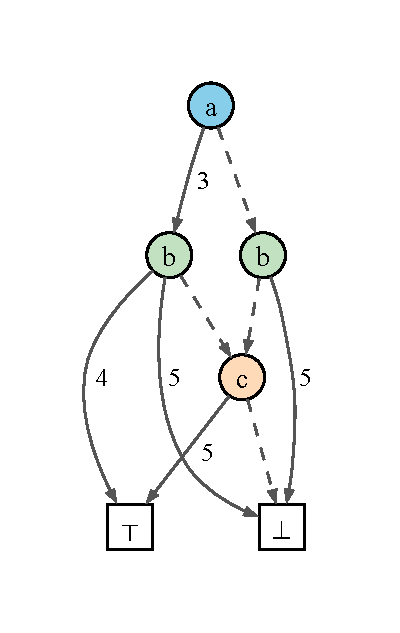
\includegraphics[scale=0.5]{viz/sp1.pdf}
        \caption{$a\test3 \cdot b\test4 \mathrel{+} b \testNE 5 \cdot c\test5$}
        \label{fig:sp1}
    \end{subfigure}
    \hfill % add some horizontal spacing
    \begin{subfigure}[b]{0.29\textwidth}
        \centering
        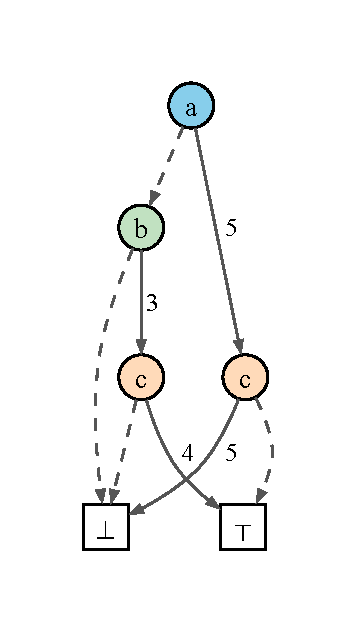
\includegraphics[scale=0.5]{viz/sp2.pdf}
        \caption{$a=3 \cdot c\test4 \mathrel{+} a\test5 \cdot c \testNE 5$}
        \label{fig:sp2}
    \end{subfigure}
    \hfill % add some horizontal spacing
    \begin{subfigure}[b]{0.40\textwidth}
        \centering
        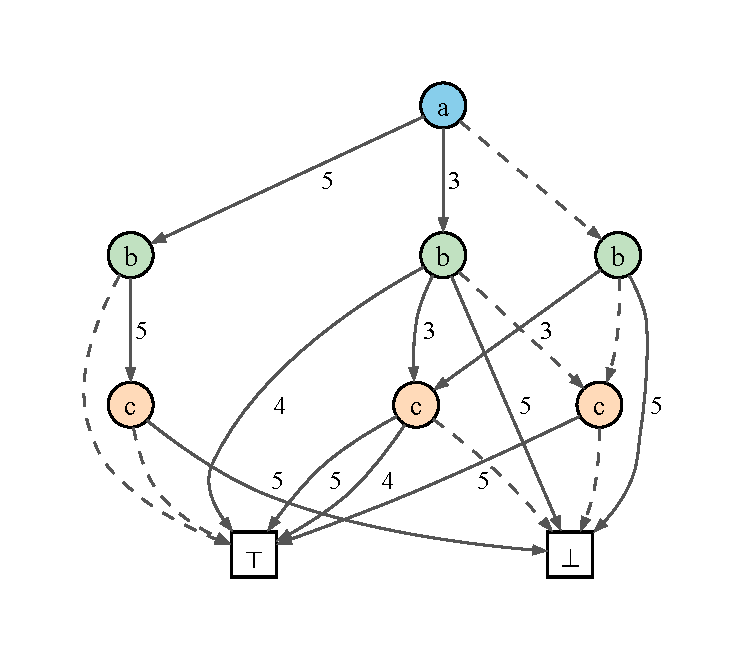
\includegraphics[scale=0.5]{viz/sp1cup2.pdf}
        \caption{Union $(\mathsf{i}) + (\mathsf{ii})$}
        \label{fig:sp1cup2}
    \end{subfigure}
    \caption{Symbolic packets}
    \label{fig:sympk}
\end{figure}

\subsection{Symbolic Transitions}\label{sec:symtrans}

We now introduce a representation for symbolic transitions in NetKAT
automata.  Whereas symbolic packets represent the fragment of NetKAT
where all atoms are tests, symbolic transitions correspond to the
larger dup-free fragment, where all atoms are tests or
assignments. This introduces additional challenges for a canonical
representation, as well as for the operations. For instance,
sequential composition is no longer equivalent to intersection, and
the star operator is no longer trivial.
\begin{align*}
    p \in \SPP \Coloneqq\ &\top \mid \bot \mid\\
    & (f = v_0) \cdot (f \mut w_{0}^{0} \cdot p_{0}^{0} + \ldots + f \mut w_{0}^{k_0} \cdot p_{0}^{k_0})\ + \\
    & \cdots \\
    & (f = v_n) \cdot (f \mut w_{n}^{0} \cdot p_{n}^{0} + \ldots + f \mut w_{n}^{k_n} \cdot p_{n}^{k_n})\ + \\
    & (f \neq v_0 \cdots f \neq v_n) \cdot (f \mut w_{n+1}^{0} \cdot p_{n+1}^{0} + \ldots + f \mut w_{n+1}^{k_{n+1}} \cdot p_{n+1}^{k_{n+1}}\ + \\
    & \phantom{(f \neq v_0 \cdots f \neq v_n) \cdot\ \ \ } f \neq w_{n+1}^{0} \cdots f \neq w_{n+1}^{k_{n+1}} \cdot f \mut w_{n+1}^{k_{n+1}+1} \cdot p_{n+1}^{k_{n+1}+1})
\end{align*}

Like SPs, \SPPn{}s have two base cases, $\top$ and $\bot$.
Also like SPs, \SPPn{}s test a field $f$ of the input packet against a series of values $v_0,\dots,v_n$, with a default case $f \neq v_0 \cdots f \neq v_n$.
However, instead of continuing recursively after the test, \SPPn{}s non-deterministically assign a value $w_i^j$ to the field $f$ of the output packet, and continue recursively with the corresponding child $p_i^j$.
This way, \SPPn{}s can output more than one packet for a given input packet, and can also output packets with different values for the same field.
The default case is further split into two cases, one where the field $f$ is non-deterministically assigned a new value (like in the other cases), and an identity case where the field $f$ keeps the same value as the input packet.
However, the packet for the latter case is not produced when the input packet's field $f$ had a value that could also be produced by the explicit assignments in the default case.
This is indicated by the test $f \neq w_{n+1}^{0} \cdots f \neq w_{n+1}^{k_{n+1}}$, and ensures that for a given input packet, a given output packet is produced by a unique path through the \SPPn{}.

The following conditions need to be satisfied for a \SPPn{} to be in canonical form:

\begin{description}
    \item[Reduced] If a child $p_i^j$ is equal to $\bot$, it is removed (with the exception of the default-identity case, which is always kept).
    If one of the default-assignment cases for a value $w$ is $\bot$, it is removed, but to keep the behavior equivalent, an additional test for the same value $w$ is added, with an empty sequence of assignments (if a test for the value $w$ was already present, nothing is added).
    Further, each of the non-default cases is analyzed, and if we determine that it behaves semantically like the default case for that input value, then it is removed.
    If only the default case remains, the \SPPn{} is reduced to the default case itself.
    \item[Ordered] A path down the tree always follows the same order of fields, and both the tests and the assignments are ordered by the value $v_i$ or $w_i^j$.
\end{description}

These conditions ensure the representation of a \SPPn{} is unique, in the sense that two \SPPn{}s are semantically equal if and only if they are syntactically equal.

\paragraph{Representation}
Like symbolic packets, we represent \SPPn{}s as a directed acyclic graph, with duplicate nodes shared.
Examples of \SPPn{}sare shown in \Cref{fig:symt}.
Vertices are labeled with the packet field that they test.
Solid arrows labeled with a number represent the tests, and dashed arrows represent the default case.
Each test is followed by a non-deterministic assignment of a new value to the field, indicated by the small diamonds.
In the default case, the non-deterministic assignment also has an identity case (keeping the value of the field unchanged), indicated by a dashed arrow emanating from the diamond.

% val sx = SPP.seq(
%   SPP.union(testS("a", 5), testS("b", 2)),
%   SPP.union(mutS("b", 1), testS("c", 5))
% )

% val sy = SPP.union(
%   SPP.union(testS("b", 1), mutS("c", 4)),
%   SPP.seq(mutS("a", 1), mutS("b", 1))
% )
\begin{figure}
    \centering
    \begin{subfigure}[b]{0.27\textwidth}
        \centering
        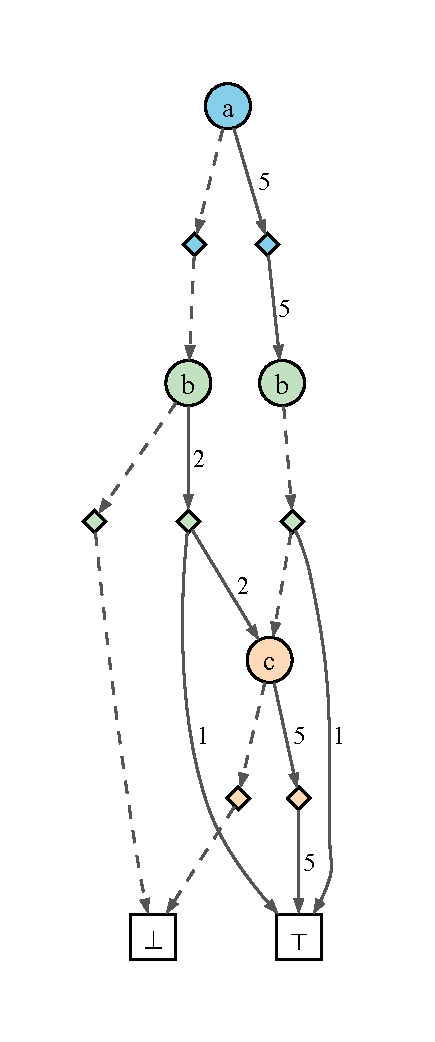
\includegraphics[scale=0.5]{viz/spp1.pdf}
        \caption{$(a \test 5 + b \test 2) \cdot (b \mut 1 + c \test 5)$}
        \label{fig:spp1}
    \end{subfigure}
    \begin{subfigure}[b]{0.33\textwidth}
        \centering
        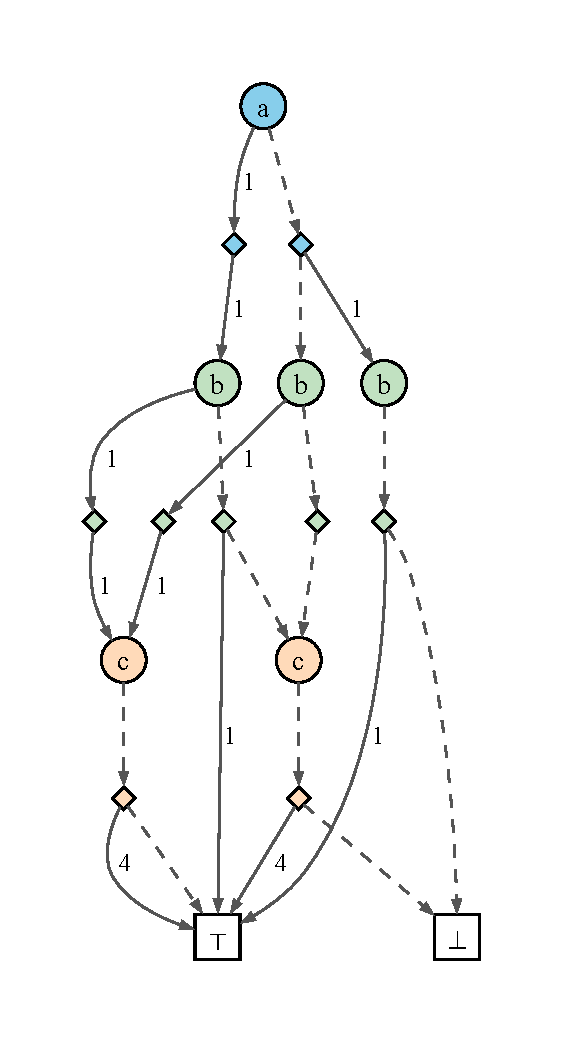
\includegraphics[scale=0.5]{viz/spp2.pdf}
        \caption{$b \test 1 \mathrel{+} c \mut 4 \mathrel{+} a \mut 1 \cdot b \mut 1$}
        \label{fig:spp2}
    \end{subfigure}
    \begin{subfigure}[b]{0.38\textwidth}
        \centering
        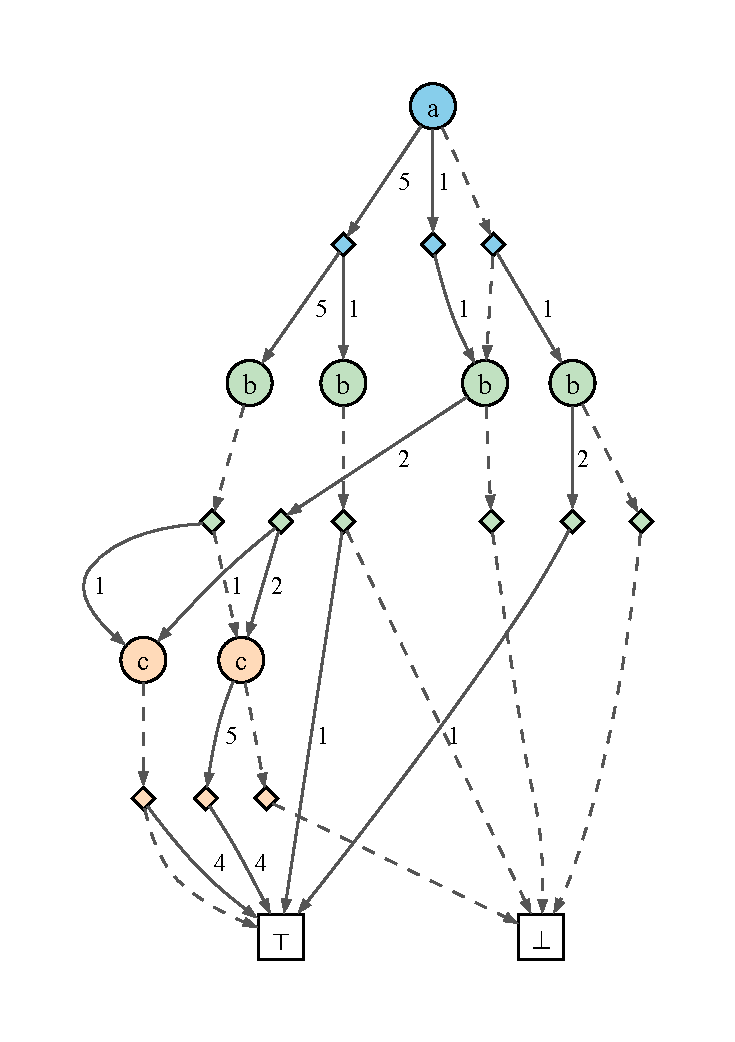
\includegraphics[scale=0.5]{viz/spp1seq2.pdf}
        \caption{Sequential composition $(\mathsf{i}) \cdot (\mathsf{ii})$}
        \label{fig:spp1seq2}
    \end{subfigure}
    \caption{Symbolic transitions represented as \SPPn{}s}
    \label{fig:symt}
\end{figure}

Let us consider the action of the first \SPPn{} in \Cref{fig:symt} on the concrete packet $a \test 5 \cdot b \test 3 \cdot c \test 5$. The first test $a \test 5$ succeeds, and the field $a$ is assigned a same value $5$. The $b$ field is then tested, but the $b$ node only has a default case. The default case does have a non-deterministic assignment, which can set the $b$ field to the new value $1$, or it can keep the old value $3$. In case the new value of $b$ is $1$, the packet is immediately accepted by the $\top$ node, so the packet $a \test 5 \cdot b \test 1 \cdot c \test 5$ is produced. In case the old value of $b$ is kept, the $c$ field is tested, and in our case the value of the $c$ field is $5$. In this case, the value of the field is unchanged, and the packet $a \test 5 \cdot b \test 3 \cdot c \test 5$ is produced.
In summary, for input packet $a \test 5 \cdot b \test 3 \cdot c \test 5$, the \SPPn{} produces the packets $a \test 5 \cdot b \test 1 \cdot c \test 5$ and $a \test 5 \cdot b \test 3 \cdot c \test 5$.

When we sequentially compose the two \SPPn{}s on the left, we get the
\SPPn{} on the right.  In other words, if we take a concrete packet,
and first apply the first \SPPn{}, and then apply the second \SPPn{}
to all of the resulting packets, then we get the same result as if we
apply the \SPPn{} on the right directly to the concrete
packet. Sequential composition is a relatively complex operation, but
algorithmically it is a key strength of our representation.  To
understand why, consider taking a concrete packet, and applying the
first \SPPn{} to it.  Once we have applied the $a$-layer of the
\SPPn{} to the packet, we already know what the value of the $a$ field
in the output packet will be.  We can therefore immediately continue
with the $a$ layer of the second \SPPn{}, without having to consider
the other layers of the first \SPPn{}.  This is in contrast to a naive
algorithm, which would have to consider the entire first \SPPn{}
before being able to apply the second \SPPn{}.  This property makes it
possible to compute the sequential composition of two \SPPn{}s
efficiently in practice, and is a key contributor to the performance
and scalability of our system.

\paragraph{Operations}
%
\SPPn{}s are closed not just under sequential composition, but under
all of the NetKAT operations.  These operations are largely
mechanical, but more complex than for SPs, as we need to take
assignments into account while respecting the conditions that ensure
uniqueness.  In particular, sequential composition is no longer
equivalent to intersection, as the assignments in the first \SPPn{}
clearly affect the tests in the second \SPPn{}.  Furthermore, the star
operator is no longer trivial, as the assignments in the \SPPn{} can
affect the tests in the \SPPn{} itself, and a fixed point needs to be
taken. We have the following operations on \SPPn{}s:
\begin{align*}
    \nf{+}, \nf{\cdot}, \nf{\cap}, \nf{\oplus}, \nf{-}\ :\ \SPP \times \SPP \to \SPP \qquad
    \nf{\star}\ :\ \SPP \to \SPP \qquad
    f \test v, f \testNE v, f \mut v \ :\ \SPP
\end{align*}

The left side of \Cref{fig:symt2} shows the result of applying the
symmetric difference to first two \SPPn{}s in \Cref{fig:symt}.  That
is, if we take a concrete packet, and first two \SPPn{}s to it, and
then take the symmetric difference of the resulting sets of packets,
we get the same result as applying the symmetric difference \SPPn{} to
the concrete packet directly.

The right side of \Cref{fig:symt2} shows the result of applying the
star operator to the result of the symmetric difference.  That is, if
we take a concrete packet, and first apply the symmetric difference
\SPPn{} to it, and then apply it again to all of the resulting
packets, iteratively until we reach a fixed point, we get the same
result as if we apply the star \SPPn{} to the concrete packet once.

\renewcommand\thesubfigure{\arabic{subfigure}}
\begin{figure}
    \centering
    \begin{subfigure}[b]{0.6\textwidth}
        \centering
        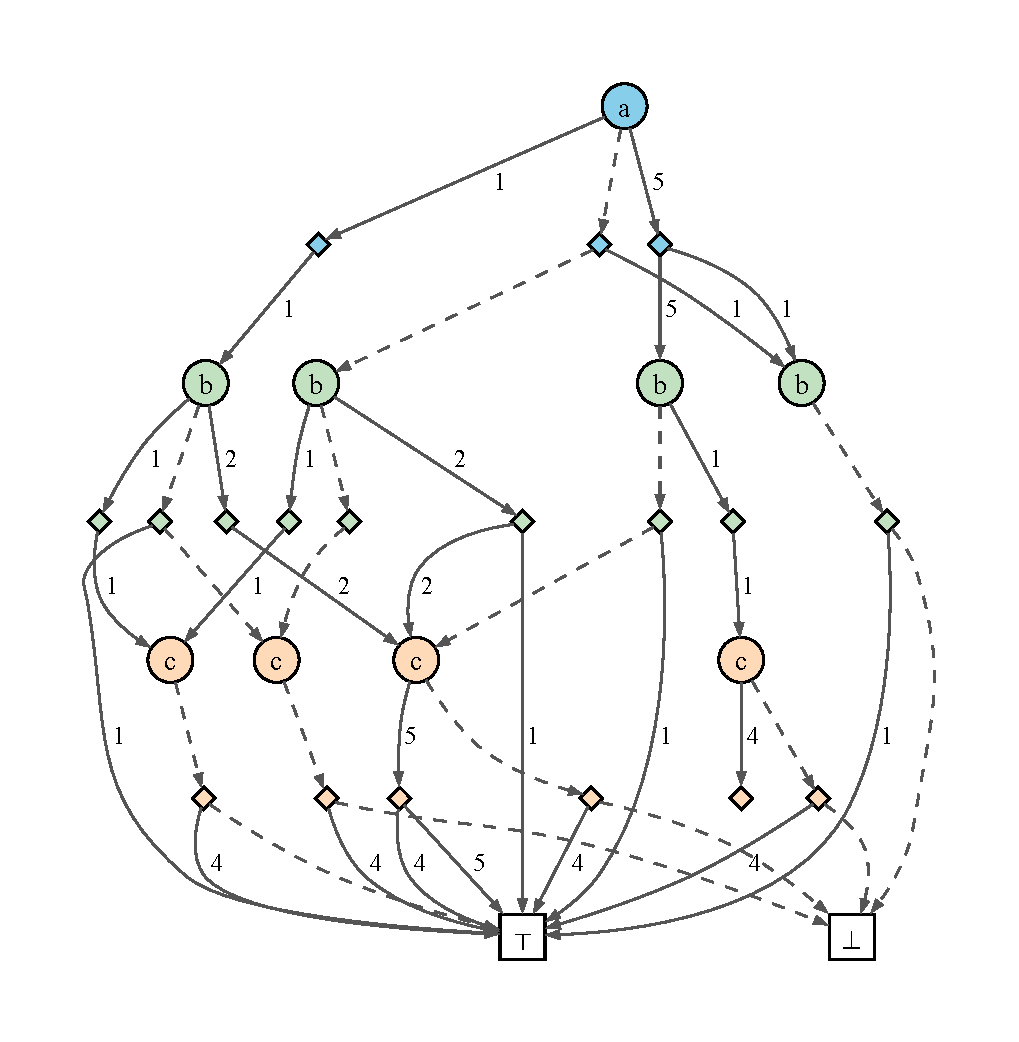
\includegraphics[scale=0.5]{viz/spp1xor2cp.pdf}
        \caption{Symmeric difference $(i) \oplus (ii)$}
        \label{fig:spp1xor2}
    \end{subfigure}
    \hfill % add some horizontal spacing
    \begin{subfigure}[b]{0.39\textwidth}
        \centering
        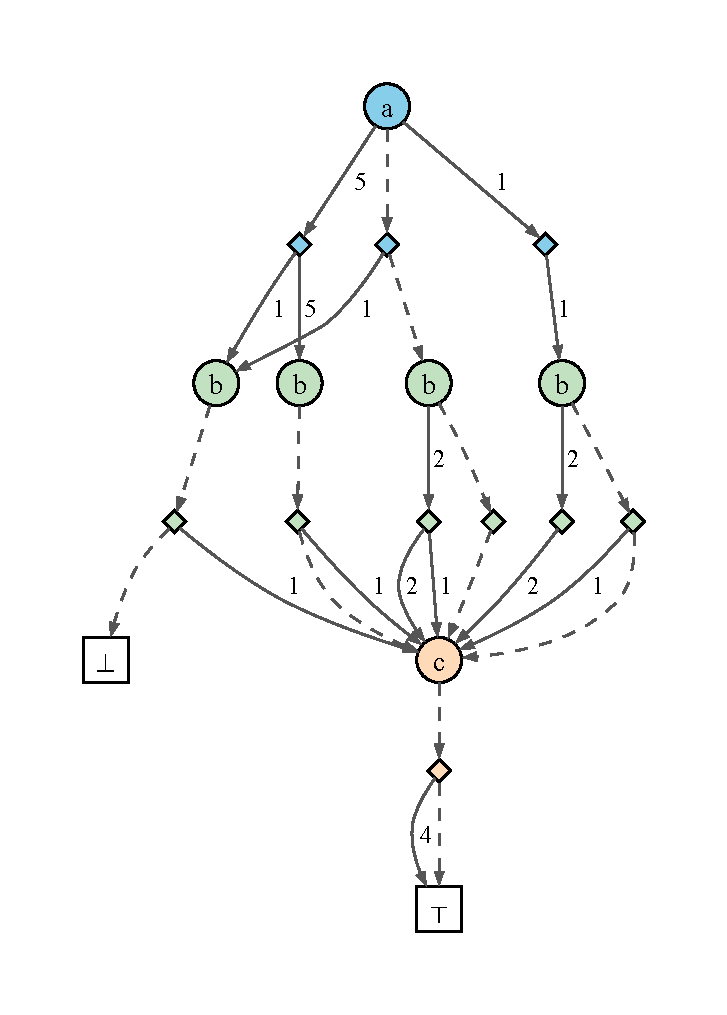
\includegraphics[scale=0.5]{viz/spp1xor2star.pdf}
        \caption{Star $((\mathsf{i}) \oplus (\mathsf{ii}))^\star$}
        \label{fig:spp1xor2star}
    \end{subfigure}
    \caption{Symbolic operations (where (i) and (ii) are from \Cref{fig:symt})}
    \label{fig:symt2}
\end{figure}

\paragraph{Push and pull}
In addition to these operations for combining \SPPn{}s, we also have
the following operations, which ``push'' and ``pull'' a symbolic
packet through a \SPPn:
\begin{align*}
    \mathsf{push} :\ \SP \times \SPP \to \SP \qquad\qquad
    \mathsf{pull} :\ \SPP \times \SP \to \SP
\end{align*}

The push operation computes the effect of a \SPPn{} on a symbolic packet, giving a symbolic packet as a result. The new symbolic packet contains all of the packets that are produced by the \SPPn{} when applied to the packets in the input symbolic packet.

The pull operation simulates the effect of a \SPPn{} in reverse.
This operation is used when computing the backward transition of a symbolic packet over a symbolic transition, for counter-example generation.
The pull operation answers this question: given a set of output packets (represented symbolically), what are the possible input packets (also represented symbolically) that could have produced them?
In other words, a concrete packet is an element of $\mathsf{pull}(p,q)$ if and only if running the \SPPn{} $p$ on the concrete packet produces a set of packets that has non-empty intersection with $q$.

\section{Symbolic NetKAT Automata via Brzozowski Derivatives}\label{sec:symaut}

With the symbolic packet and symbolic transition representations in
place, we can now define symbolic NetKAT automata.  The construction
of NetKAT automata shares some similarities with the construction of
automata for regular expressions.  In prior
work~\cite{Foster2015,Smolka2015}, NetKAT automata were constructed
via Antimirov derivatives \cite{Antimirov1996}, which can be extended
from regular expressions to NetKAT.  The Antimirov derivative
constructs a non-deterministic automaton, and as such, is well suited
for handling \NetKAT's union operator by inserting transitions for the
two sub-terms.  However, the Antimirov derivative is not well suited
for our extended set of logical operators, as we cannot simply insert
(non-deterministic) transitions for the operands of intersection,
difference, and symmetric difference.  Instead, we extend the
Brzozowski derivative \cite{Brzozowski1962} to NetKAT, which
constructs a deterministic automaton directly, and is better suited
for the logical operators.

In the rest of this section, we will first describe what symbolic
NetKAT automata are, and then describe how to construct them via the
Brzozowski derivative.

\subsection{Symbolic NetKAT Automata}

An automaton for a regular expression consists of a set of states, and
transitions labeled with symbols from the alphabet.  Additionally, one
of the states is designated as the initial state, and a subset of the
states are designated as accepting states.  This way, an automaton for
a regular expression models the set of strings that are accepted by
the regular expression.

An automaton for a NetKAT program is similar, but instead of modeling
a set of strings, it models the traces that are produced for a given
input packet.  When a packet travels through the automaton, every
state that it traverses acts as a $\text{dup}$ operation, appending a
copy of the packet to the packet's trace.  Therefore, the transition
between two states is labeled with a dup-free NetKAT program,
represented symbolically as a \SPPn{}.  Secondly, instead of having a
boolean at each state that determines whether it is accepting or not,
NetKAT automata have a additional \SPPn{} at each state that
determines the set of packets that are produced as output of the
automaton when a packet reaches that state.  Therefore, a symbolic
NetKAT automaton consists of the following data:
\begin{description}
    \item[States] A set of states $Q$.
    \item[Initial state] A state $q_0 \in Q$.
    \item[Transitions] A function $\delta : Q \times Q \to \SPP$.
    \item[Output] A function $\epsilon : Q \to \SPP$.
\end{description}

\paragraph{Deterministic NetKAT automata}
%
The notion of deterministic NetKAT automaton is more subtle than for
regular expressions.  For regular expressions, a deterministic
automaton is one where for every state $q$ and symbol $a$, there is at
most one transition from $q$ labeled with $a$.  For a NetKAT
automaton, we need to take into account the fact that the transitions
are labeled with \SPPn{}s, which may produce multiple packets for a
given input packet.  Therefore, we define a deterministic NetKAT
automaton as one where for every state $q$ and packet $\pk$, the set
of packets produced by $\mathsf{push}(\pk,\delta(q,q'))$ are disjoint
for all $q' \in Q$.  This is equivalent to saying that $\delta(q,q_1')
\mathop{\nf{\cap}} \delta(q,q_2') = \bot$ for all $q_1',q_2' \in Q$
($q_1' \neq q_2'$).  Note that an input packet $\pk$ may produce
multiple different packets at each successor state, but these packet
sets at different successor states are disjoint.

\subsection{Constructing Automata via Brzozowski Derivatives}

We now describe how to construct a symbolic NetKAT automaton for a
NetKAT program via the Brzozowski derivative.  We take the set of
states to be the set of NetKAT expressions, and the initial state to
be the NetKAT program itself.  Because we want to construct a
deterministic automaton, we need a way to represent a non-intersecting
outgoing symbolic transition structure (STS).  We represent such a
transition structure as a NetKAT expression in the following form:
\begin{align*}
    r \in \mathsf{STS} \Coloneqq p_1 \cdot \mathrel{\text{dup}} \cdot\ q_1 + \ldots + p_n \cdot \mathrel{\text{dup}} \cdot\ q_n
\end{align*}
where $p_i \in \SPP$ are \SPPn{}s, and $q_i \in \mathsf{Exp}$ are NetKAT expressions.
Furthermore, we require that the $p_i$ are pairwise disjoint, that is, $p_i \mathop{\nf{\cap}} p_j = \bot$ for all $i \neq j$.

\paragraph{Operations}
%
The dup operation itself is an STS, by taking $r = \top \cdot
\text{dup} \cdot \top$.

We extend the logical operators of extended NetKAT to STSs:
\begin{align*}
    \tilde{+}, \tilde{\cap}, \tilde{\oplus}, \tilde{-}\ :\ \mathsf{STS} \times \mathsf{STS} \to \mathsf{STS}
\end{align*}
These operations need to be defined such that the resulting STS is deterministic.
For instance, for $r_1 \cap r_2$, consider the following construction:
\begin{align*}
    (p_1 \cdot \text{dup} \cdot q_1 + \ldots + p_n \cdot \text{dup}\ \cdot q_n) \mathrel{\tilde{\cap}} (p'_1 \cdot \text{dup} \cdot q'_1 + \ldots + p'_n \cdot \text{dup} \cdot q'_n)
\end{align*}
To bring this in STS form, we distribute the intersection over the union, and combine the terms:
\begin{align*}
    (p_1 \mathop{\nf{\cap}} p'_1) \cdot \text{dup} \cdot (q_1 \cap q'_1) +
    (p_1 \mathop{\nf{\cap}} p'_2) \cdot \text{dup} \cdot (q_1 \cap q'_2) +
    \ldots +
    (p_n \mathop{\nf{\cap}} p'_n) \cdot \text{dup} \cdot (q_n \cap q'_n)
\end{align*}
This is not yet in STS form, as the $q_i \cap q'_i$ terms may not all be different, so we need to collect the terms with the same $q_i \cap q'_i$, and union their \SPPn{}s.
The other operators need a similar (albeit slightly more complicated) treatment in order to maintain determinism.

Second, we extend sequential composition to STSs, in two forms (denoted with the same symbol).
We can compose an STS with a \SPPn{} on the left, or with a NetKAT expression on the right:
\begin{align*}
    \tilde{\cdot} : \SPP \times \mathsf{STS} \to \mathsf{STS} \qquad
    \tilde{\cdot} : \mathsf{STS} \times \mathsf{Exp} \to \mathsf{STS}
\end{align*}
Like the other operators, these need to be defined such that the resulting STS is deterministic.

All of the STS operations are defined in terms of \SPPn{} operations.
Therefore, an efficient \SPPn{} implementation is a key component of our system,
not only for the operations on symbolic packets, but also for the operations on STSs that are used to construct the NetKAT automaton.

\paragraph{Brzozowski derivative}
With these operations in place, it is straightforward to define the Brzozowski derivative for NetKAT expressions:

\begin{minipage}{0.5\textwidth}
    \begin{align*}
        \epsilon(p + q) &\triangleq \epsilon(p) \mathop{\nf{+}} \epsilon(q) \\
        \epsilon(p \cap q) &\triangleq \epsilon(p) \mathop{\nf{\cap}} \epsilon(q) \\
        \epsilon(p \oplus q) &\triangleq \epsilon(p) \mathop{\nf{\oplus}} \epsilon(q) \\
        \epsilon(p - q) &\triangleq \epsilon(p) \mathop{\nf{-}} \epsilon(q) \\
        \epsilon(p \cdot q) &\triangleq \epsilon(p) \mathop{\nf{\cdot}} \epsilon(q) \\
        \epsilon(p^\star) &\triangleq \epsilon(p)^\star \\
        \epsilon(\text{dup}) &\triangleq \bot\\
        \epsilon(f \test v) &\triangleq f \test v\\
        \epsilon(f \testNE v) &\triangleq f \testNE v\\
        \epsilon(f \mut v) &\triangleq f \mut v\\
        \epsilon(\top) &\triangleq \top\\
        \epsilon(\bot) &\triangleq \bot
    \end{align*}
\end{minipage}
\begin{minipage}{0.5\textwidth}
\begin{align*}
    \delta(p + q) &\triangleq \delta(p) \mathop{\tilde{+}} \delta(q) \\
    \delta(p \cap q) &\triangleq \delta(p) \mathop{\tilde{\cap}} \delta(q) \\
    \delta(p \oplus q) &\triangleq \delta(p) \mathop{\tilde{\oplus}} \delta(q) \\
    \delta(p - q) &\triangleq \delta(p) \mathop{\tilde{-}} \delta(q) \\
    \delta(p \cdot q) &\triangleq
        \delta(p) \mathop{\tilde{\cdot}} q \mathrel{\tilde{+}}
        \epsilon(p) \mathop{\tilde{\cdot}} \delta(q) \\
    \delta(p^\star) &\triangleq \delta(p) \mathrel{\tilde{\cdot}} p^\star \\
    \delta(\text{dup}) &\triangleq \tilde{\dup}\\
    \delta(f \test v) &\triangleq \bot\\
    \delta(f \testNE v) &\triangleq \bot\\
    \delta(f \mut v) &\triangleq \bot\\
    \delta(\top) &\triangleq \bot\\
    \delta(\bot) &\triangleq \bot
\end{align*}
\end{minipage}
\medskip

We construct a deterministic symbolic NetKAT automaton for a NetKAT program $p$ as follows:
\begin{description}
    \item[States] $Q \triangleq \mathsf{Exp}$.
    \item[Initial state] $q_0 \triangleq p$.
    \item[Transitions] take $\delta(q,q')$ to be the \SPPn{} of $q'$ in the Brzozowski derivative of $\delta(q)$.
    \item[Output] $\epsilon : Q \to \SPP$, defined above.
\end{description}
The Brzozowski derivative is guaranteed to transitively reach only finitely many essentially different NetKAT expressions from a given start state.
Therefore, in the actual implementation, we do not use the infinite set $\mathsf{Exp}$ for the states, but instead use only the finitely many essentially different NetKAT terms reached from the start state.

\paragraph{Example}
Consider the following NetKAT program:
\begin{align*}
% val e = parse("(((@a←1 ⋅ @b←2 ⋅ @c←3 ⋅ δ)⋆) + ((@b=2 ⋅ @c=3 ⋅ δ)⋆))⋆")
    p \triangleq \left((a \mut 1 \cdot b \mut 2 \cdot c \mut 3 \cdot \text{dup})^\star + (b \test 2 \cdot c \test 3 \cdot \text{dup})^\star\right)^\star
\end{align*}
The NetKAT automaton for this program is shown in \Cref{fig:exaut}.
The edges are labeled with the \SPPn{}s that represent the transitions.
The output \SPPn{} of every state is $\top$, i.e., the automaton accepts all packets that reach a state.

\begin{figure}
    \centering
    \begin{subfigure}[b]{0.4\textwidth}
        
\includegraphics[scale=0.5]{deriv/deriv.pdf}
        \caption*{NetKAT automaton}
    \end{subfigure}
    \begin{subfigure}[b]{0.16\textwidth}
        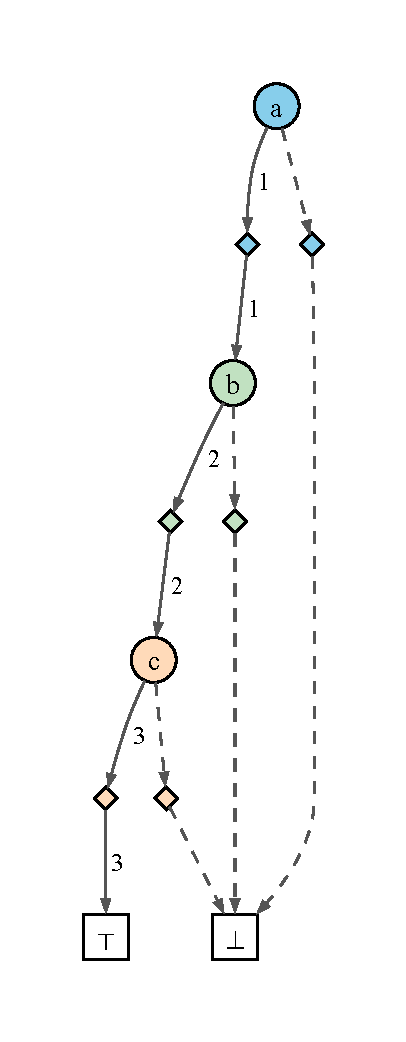
\includegraphics[scale=0.45]{deriv/derivsppA.pdf}
        \caption*{A}
    \end{subfigure}
    \begin{subfigure}[b]{0.25\textwidth}
        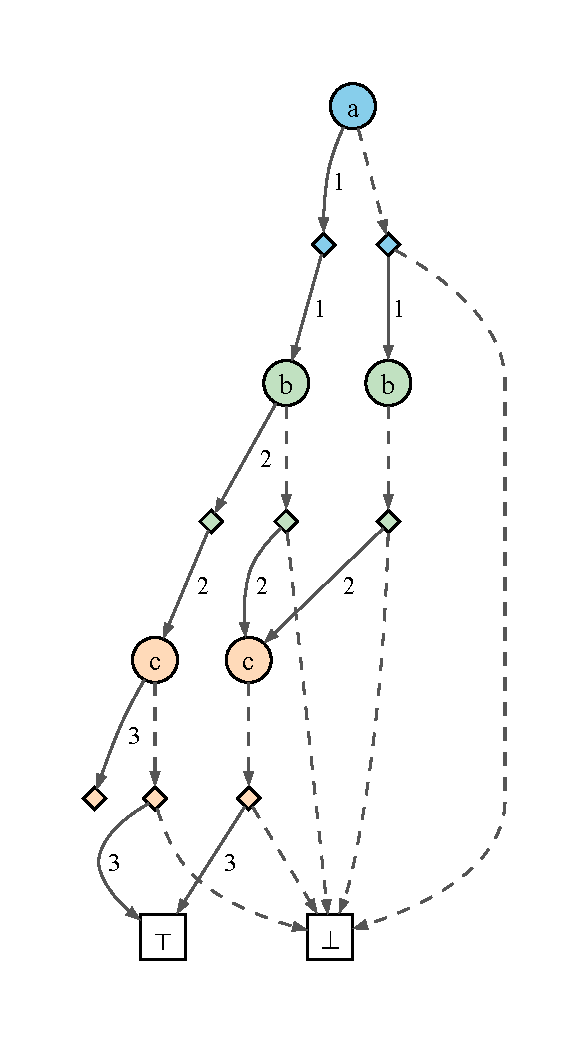
\includegraphics[scale=0.45]{deriv/derivsppB.pdf}
        \caption*{B}
    \end{subfigure}
    \begin{subfigure}[b]{0.16\textwidth}
        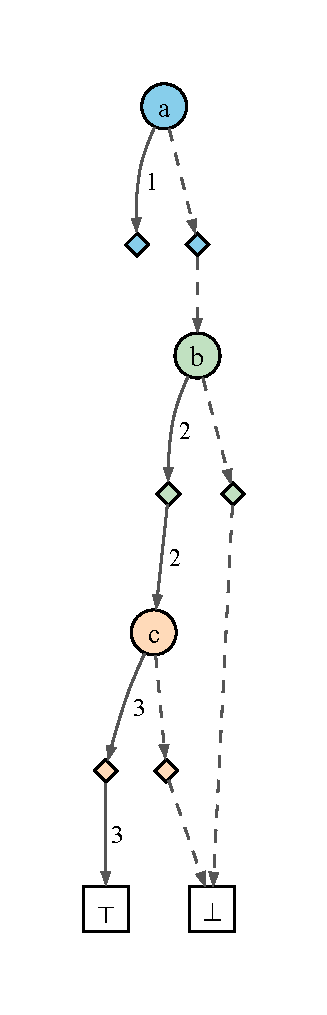
\includegraphics[scale=0.45]{deriv/derivsppC.pdf}
        \caption*{C}
    \end{subfigure}
    \caption{Symbolic NetKAT automaton for $p \triangleq \left((a \mut 1 \cdot b \mut 2 \cdot c \mut 3 \cdot \text{dup})^\star + (b \test 2 \cdot c \test 3 \cdot \text{dup})^\star\right)^\star$}
    \label{fig:exaut}
\end{figure}

\section{Bisimilarity and Counter-Example Generation}\label{sec:fwdbwd}

Historically, methods for computing bisimulations of automata
\cite{Bonchi2013,Doenges2022} have been based on either on Moore's
algorithm for minimization \cite{Moore1956} or Hopcroft and Karp's
algorithm \cite{Hopcroft1971}. Indeed, the naive approach shown
in \Cref{fig:bisim} follows the basic structure of Hopcroft-Karp, in
the sense that it relates the start states and proceeds to follow
transitions forward in the two automata.

Our situation is different, because we have already added the
symmetric difference operator to NetKAT.  Therefore, we can reduce
equivalence checks $A \equiv B$ to emptiness checks $A \oplus B \equiv
\bot$.

\paragraph{Subtlety of symmetric difference}
%
The reader should note that the situation is a bit more subtle than it
may seem at first sight.  In particular, consider the query $A \equiv
B$, which asks whether two NetKAT programs $A$ and $B$ are equivalent.
If they are inequivalent, then there must be some input packet that
causes $A$ to produce a different output than $B$.  Output in this
sense does not just mean the final output packet, but also the trace
of the packet.  It can be the case that $A$ and $B$ produce the same
final output packets, but differ in the trace of the packets.
Therefore, the symmetric difference $A \oplus B$ takes the symmetric
difference of the traces, not just of the output packets, i.e., the
symmetric difference $A \oplus B$ contains precisely the traces of the
packets that are produced by $A$ or $B$, but not by both.  In other
words, the symmetric difference $A \oplus B$ contains precisely the
traces that are counter-examples to the equivalence of $A$ and $B$.

\paragraph{Subtlety of the emptiness of an automaton}
%
A second subtlety is the emptiness of an automaton.  Whereas for
regular expressions, it is easy to check whether a DFA is empty (just
check whether there are \emph{any} accepting states), this is not the
case for NetKAT automata.  Because NetKAT automata manipulate and test
the fields of packets, it is possible that a packet travels through
the automaton, and even causes multiple packets to be produced (e.g.,
due to the presence of union in the original NatKAT expression), but
nevertheless, it is possible that all of these packets eventually
dropped by the automaton, before producing any output packets.

The goal of this section is to develop a symbolic algorithm for this
check, which is more efficient than the naive algorithm that checks
all concrete input packets separately.

\subsection{Forward Algorithm}

To check whether a NetKAT automaton drops all input packets, we
develop a \emph{forward algorithm}.  The forward algorithm computes
\emph{all} output packets that the automaton can produce, across all
possible input packets.  The forward algorithm therefore starts with
the complete symbolic packet $\top$ at the input state, and repeatedly
applies all outgoing transitions $\delta$ to it.  In this way, the
algorithm iteratively accumulates a symbolic packet at every state,
which represents the set of packets that can reach that state from the
start state.  Once we know the set of packets that can reach a state,
we can determine the set of output packets by applying the output
function $\epsilon$ to the symbolic packet of each state, and taking
the union of the results.

\newcommand{\pluseq}{\mathrel{\nf{+}}=}
\begin{figure}
    \begin{subfigure}[t]{0.49\textwidth}
    \begin{algorithmic}
    % \State \textbf{Input:} A NetKAT automaton $(Q, q_0, \delta, \epsilon).$
    % \State \textbf{Returns:} The symbolic set of output packets that the automaton can produce.\\
    \State $\doneR(q) \gets \bot \text{ for } q \in Q$;
    \State $\todoR(q) \gets \bot \text{ for } q \in Q \setminus \{q_0\}$;
    \State $\todoR(q_0) \gets \top$;
    \While{$\exists q.\ \todoR(q) \neq \bot$}
        \State set $p := \todoR(q) \mathrel{\nf{-}} \doneR(q)$;
        \State $\todoR(q) \gets \bot$;
        \State $\doneR(q) \pluseq p$;
        \For {$q' \in Q$}
            \State $\todoR(q') \pluseq \mathsf{push}(p,\delta(q,q'))$;
          \EndFor
    \EndWhile
    \State
    \Return $\sum_{q \in Q} \mathsf{push}(\doneR(q), \epsilon(q))$;
    % \mathrel{\nf{+}} \cdots \mathrel{\nf{+}} \mathsf{push}(\doneR(q_n), \epsilon(q_n))$;
    \end{algorithmic}
    \caption{Forward algorithm}
    \end{subfigure}
    \begin{subfigure}[t]{0.49\textwidth}
    \begin{algorithmic}
    % \State \textbf{Input:} a NetKAT automaton $(Q, q_0, \delta, \epsilon).$
    % \State \textbf{Returns:} The symbolic set of input packets that the automaton does not drop.\\
    \State $\doneR(q) \gets \bot \text{ for } q \in Q$;
    \State $\todoR(q) \gets \mathsf{pull}(\epsilon(q), \top) \text{ for } q \in Q$;
    \State
    \While{$\exists q.\ \todoR(q) \neq \bot$}
        \State set $p := \todoR(q) \mathrel{\nf{-}} \doneR(q)$;
        \State $\todoR(q) \gets \bot$;
        \State $\doneR(q) \pluseq p$;
        \For {$q' \in Q$}
            \State $\todoR(q') \pluseq \mathsf{pull}(\delta(q',q), p)$;
          \EndFor
    \EndWhile
    \State
    \Return $\doneR(q_0)$;
    \end{algorithmic}
    \caption{Backward algorithm}
    \end{subfigure}
    \caption{Forward and backward algorithms for NetKAT automata}
    \label{fig:forward}
    \label{fig:backward}
\end{figure}

The forward algorithm is shown in \Cref{fig:forward}.  To determine
the set of packets that a given NetKAT expression $p$ can produce, we
convert it to a NetKAT automaton, and then use the forward algorithm
to determine the symbolic output packet.  In our implementation, we
also have a way to stop the algorithm early, if the user is only
interested in a ``yes'' or ``no'' answer for the query $p \equiv
\bot$. In this case, we can stop the algorithm as soon as any output
packet is produced.

\subsection{Backward Algorithm}

The forward algorithm gives us the set of output packets that a NetKAT
automaton can produce, but we are also interested in which input
packets cause this output to be produced.  For a given check $A \equiv
B$, we want to know \emph{which} input packets cause $A$ and $B$ to
produce different sets of output traces.  More generally, for a NetKAT
automaton, we want to know which input packets cause the automaton to
produce a non-empty set of output packets.

To answer this question, we developed a \emph{backward algorithm},
shown in \Cref{fig:backward}.  The backward algorithm computes
\emph{all} input packets that can cause the automaton to produce a
non-empty set of output packets.  The backward algorithm therefore
starts with the complete symbolic packet $\top$ at every state, and
pulls it backwards through all output transitions $\epsilon$.  The
algorithm then iteratively accumulates a symbolic packet at every
state, which represents the set of packets that will cause the
automaton to produce a non-empty set of output packets, when starting
from that state.  The accumulation is done by pulling the symbolic
packet backwards through all transitions $\delta$, until fixpoint is
reached.  Once fixpoint is reached, we simply return the symbolic
packet at the start state, which represents the set of input packets
that will cause the automaton to produce a non-empty set of output
packets when starting from the start state.

\section{Implementation}\label{sec:impl}

We have implemented the algorithms in a new system, \KATch{}, comprising
2500 lines of Scala. In this section we explain the system's interface, and in the next section we evaluate its performance.% and provide details of what makes the implementation efficient.

\begin{figure}
    \centering
    \begin{tabular}{c l l l}
        % \textbf{Syntax} & & \\
        % \hline
        \text{Statements} $c$ $\Coloneqq$ & $\NKcheck\ e_1\
        (\equiv\mid\nequiv)\ e_2$ & Check equivalence or inequivalence\\
                        & $\NKprint\ e$ & Pretty print\\
                        & $x = e$ & Let\\
                        & $\NKimport$ ``\emph{filename}'' & Import NKPL file\\
                        & $\NKfor\ i\ \in n_1..n_2\ \NKdo\ c$ & For loop\\[2mm]
        \text{Expressions} $e$ $\Coloneqq$ & $\NKforward\ e$ & Compute symbolic packet forward\\
                        & $\NKbackward\ e$ & Compute symbolic packet backward\\
                        & $e_1 \cap e_2$ & Intersection\\
                        & $e_1 \oplus e_2$ & Symmetric difference (xor)\\
                        & $e_1 - e_2$ & Set difference\\
                        & $f \in n..m$ & Range test; sugar for $f \test n + \cdots + f \test m$\\
                        & $\NKexists\ f\ e$ & Existential quantifier for symbolic packet $e$\\
                        & $\NKforall\ f\ e$ & Universal quantifier for symbolic packet $e$ \\
                        & $p$ & \NetKAT Program Expression (in \Cref{fig:synsem})\\
    \end{tabular}
    \caption{Syntax for \NetKAT Programming Language (NKPL).}
\label{fig:nknf}
\end{figure}

The implementation provides a surface syntax for expressing queries,
which extends the core \NetKAT syntax from \Cref{fig:synsem}. The extended
syntax is shown in \Cref{fig:nknf}.
The language has statements and expressions, which we describe below.

\paragraph*{Statements}
The $\NKcheck\ e_1 \equiv e_2$ command runs the bisimulation algorithm (in the forward
direction). The system reports success if the expressions are equivalent (when
$\equiv$ is used) or inequivalent (when $\nequiv$) is used, or reports failure
otherwise. The other statements behave as expected:
The $\NKprint$ statement invokes the pretty printer,
$\NKlet$ binds names to expressions,
$\NKimport$ runs the named file making its bound names available,
and $\NKfor$ run a statement in a loop.

\paragraph*{Expressions}
The $\NKforward\ e$ expression computes, in forward-flowing mode, the set of
output packets resulting from running the symbolic packet $\top$ through the given
expression $e$ (see \Cref{fig:forward}). Conversely $\NKbackward\ e$ computes the set of input packets which
generate some output packet when run on the given expression (\Cref{fig:backward}).
These are generally used in conjunction with the $\oplus, -, \cap$ operators to
express the desired query. The user may combine these expressions with the
$\NKexists$ and $\NKforall$ operators to reason about symbolic packets, and the
$\NKprint$ operator to pretty print the symbolic packets, or the $\NKcheck$
operator to assert (in)equivalence of two expressions.

We note that the generality of the language allows us to express some queries in
different, equivalent ways. For example, the two checks:
\begin{align*}
e_1 \equiv e_2 && e_1 \oplus e_2 \equiv \zero
\end{align*}
are equivalent. However, the expression on the right lends it self to
inspection of counterexample input packets:
\[ \NKprint\ (\NKbackward\ e_1 \oplus e_2). \]
This statement pretty prints a symbolic representation of all packets that have
different behavior on $e_1$ and $e_2$ (i.e., result in some valid history in one
expression and not the other). In other words, the command prints the set of all
counter-example input packets for the query $e_1 \equiv e_2$.

% Another way to understand $\NKexists$ and $\NKforall$, is that given an
% expression with tests, $\NKexists\ f$ replaces all $f=v_i$ with $\one$ and $\NKforall$
% replaces all tests $f=v_i$ with $\zero$. For example:
% \begin{align*}
% \NKexists\ \sw\ (\sw=3\cdot \pt=2 \cup \sw=1\cdot \pt=3) \equiv \pt=2 \cup \pt=3\\
% \NKforall\ \sw\ (\sw=3\cdot \pt=2 \cup \sw=1\cdot \pt=3) \equiv \zero\\
% \end{align*}


\paragraph{Topologies and routing tables}
While NetKAT can be used to specify routing policies declaratively, it is also possible to import topologies and routing tables into NetKAT.
For example, a simple way to define routing tables and topologies in NetKAT is as follows:
% \begin{align*}
%     \mathsf{route} \triangleq\ &\sw \test 5 \cdot (\dst \test 6 \cdot \pt \mut 3 + \dst \test 8 \cdot \pt \mut 4)\ + \\
%         & \sw \test 6 \cdot (\dst \test 5 \cdot \pt \mut 2 + \dst \test 8 \cdot \pt \mut 3)\ + \\
%         &\cdots\\
%         & \sw \test 7 \cdot (\dst \test 8 \cdot \pt \mut 2 + \dst \test 9 \cdot \pt \mut 1) \\[1em]
%     \mathsf{topo} \triangleq\ &\sw \test 5 \cdot (\pt=3 \cdot \sw \mut 6 + \pt=4 \cdot \sw \mut 8)\ + \\
%         & \sw \test 6 \cdot (\pt=2 \cdot \sw \mut 5 + \pt=3 \cdot \sw \mut 8)\ + \\
%         &\cdots\\
%         & \sw \test 7 \cdot (\pt=2 \cdot \sw \mut 8 + \pt=1 \cdot \sw \mut 9)
% \end{align*}

\medskip
\noindent
\begin{tabular}{lc@{\ \ \ \ }|@{\ \ \ \ }lc}

    $\mathsf{R} \triangleq$\!\!\!\!&$\sw \test 5 \cdot (\dst \test 6 \cdot \pt \mut 3 + \dst \test 8 \cdot \pt \mut 4)$&
    $\mathsf{T} \triangleq$\!\!\!\!&$\sw \test 5 \cdot (\pt=3 \cdot \sw \mut 6 + \pt=4 \cdot \sw \mut 8)$ \\
%
        % &$ \sw \test 6 \cdot (\dst \test 5 \cdot \pt \mut 2 + \dst \test 8 \cdot \pt \mut 3)\ + $ &
        % &$ \sw \test 6 \cdot (\pt=2 \cdot \sw \mut 5 + \pt=3 \cdot \sw \mut 8)\ +$ \\
%
        &$+\ \cdots\ +$&
        &$+\ \cdots\ +$\\
%
        &$ \sw \test 7 \cdot (\dst \test 8 \cdot \pt \mut 2 + \dst \test 9 \cdot \pt \mut 1) $&
        &$ \sw \test 7 \cdot (\pt=2 \cdot \sw \mut 8 + \pt=1 \cdot \sw \mut 9)$
\end{tabular}
\medskip

The routing $\mathsf{R}$ tests the switch field (where the packet currently is), and the destination field (where the packet is supposed to end up), and then sets the port over which the packet should be sent out.
The topology $\mathsf{T}$ tests the switch and port fields, and then transports the packet to the next switch.
We define the action of the network by composing the route and topology:
\begin{align*}
    \mathsf{net} \triangleq \mathsf{R} \cdot \mathsf{T} \cdot \text{dup}
\end{align*}
We include a dup to extend the trace of the packet at every hop.

\begin{example}[All-Pairs Reachability Queries]\label{ex:linear-reachability}
A naive way to check reachability of all pairs of hosts in a network is to run
the following command for each pair of end hosts $n_i$, $n_j$:
\[ \NKcheck\ (\sw \test n_i) \cdot \textsf{net}^\star \cdot (\sw \test n_j) \nequiv \bot \]
% \[ \NKcheck\ \sw=n_i \cdot (p\cdot t\cdot \dup)^\star \cdot \sw=n_j \nequiv \emptyset \]

Of course, this requires a number of queries which is quadratic in the number of
hosts---quickly becoming prohibitive. One might think that we could reduce the number of queries to $n$ by running:
\begin{align*}
    % &\textsf{net} = (p\cdot t\cdot\dup)^\star\\
    &\NKfor\ i \in 1..n\ \NKdo\ \NKcheck\ (\NKforward\ (\sw \test i \cdot \textsf{net}^\star)) \equiv (\sw \in 1..n)
\end{align*}
This query does work if $\sw$ is the only field of our packets, because the left hand side contains the packets that can be reached from $i$ via the network, and the right hand side contains packets where the $\sw$ field is any value in $1..n$.
Unfortunately, this does not quite work if the network also operates on other packet fields, as the packets on the left hand side will have those fields, whereas the packets on the right hand side will only have a $\sw$ field.
The exists and forall operators allow us to manipulate symbolic packets and give us a way to do all pairs reachability with only $n$ queries:
\begin{align*}
    % &\textsf{net} = (p\cdot t\cdot\dup)^\star\\
    &\NKfor\ i \in 1..n\ \NKdo\ \NKcheck\ (\NKexists\ f_1\ (\NKexists\ f_2\
    (\NKforward\ (\sw=i \cdot \textsf{net}^\star)))) \equiv (\sw \in 1..n)
\end{align*}

The operators $\NKexists$ and $\NKforall$ give the programmer the ability to
reason about symbolic packets that may be computed, for instance, by $\NKforward$ or
$\NKbackward$. The specifications are:
\begin{align*}
    \NKexists\ f\ e = \bigcup_{v\in V} f=v \cdot e \qquad
    \NKforall\ f\ e = \bigcap_{v\in V} f=v \cdot e
\end{align*}
The implementation does not iterate over $V$ (indeed, we need not even
know $V$). Rather, $\NKexists$ and $\NKforall$ are implemented directly as operations on symbolic packets.
In fact, the implementation does not need to fix the set of fields or the set of values up-front at all, and instead operate on a conceptually infinite set of fields and values.
This works because \SPPn{}s' default cases handle all remaining fields and all values.
\end{example}

% Motivation: From Counter examples packet to counter examples path
% Our bisimulation algorithm computes a symbolic packet (or set of
% packets) on which the two policies differs. We can use this to
% generate counter example packets to equivalence of policies: any
% packet matching the series of test between the root and a $\top$ leaf
% will be treated differently by the two policies. It may be hard to
% diagnose what is causing the different treatment as it only represents
% packets at the initial state rather that how they are routed and
% updated by the potentially non-deterministic policies. We have
% extended our backward algorithm implementation with provenance
% information, and are using it to generate paths through the network
% exemplifying their routing from the initial state to a state where
% their routing policies are immediately different, providing deeper
% insight into ways in which two policies differ.

\begin{figure}
    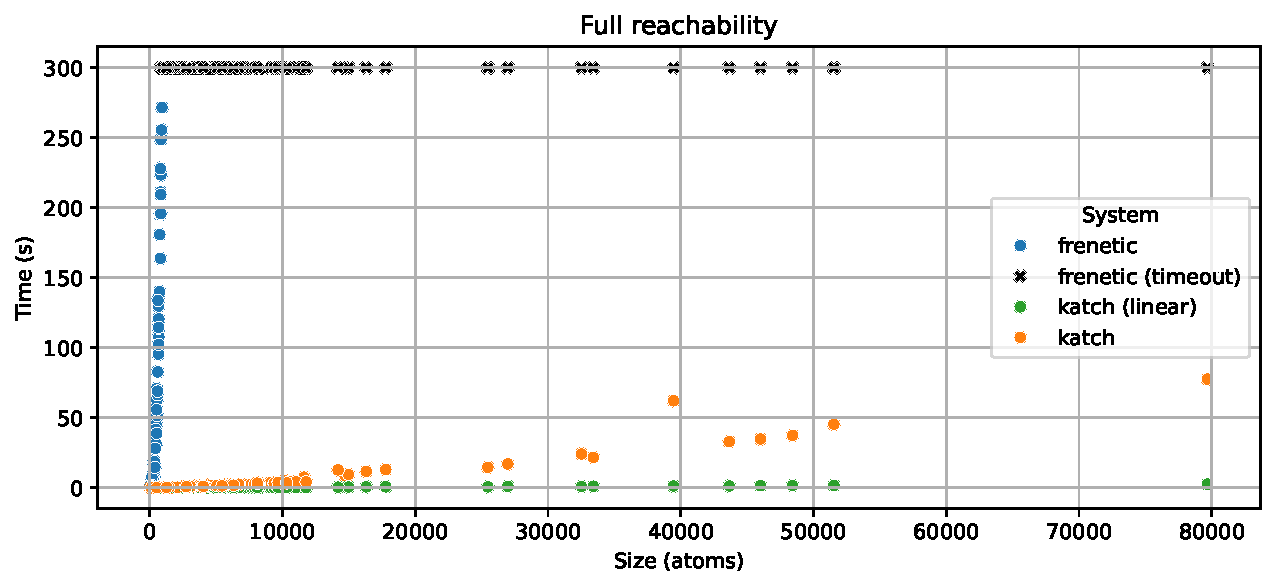
\includegraphics[scale=0.6]{plots/Full reachability_time_vs_size_wide.pdf}
    \caption{Full reachability queries on Topology Zoo}\label{fig:topology-zoo-full}
\end{figure}

\section{Evaluation}\label{sec:eval}

To evaluate \KATch{}, we conducted experiments in which we used it to
solve a variety of verification tasks for a range of topologies and
routes, as well as challenging combinatorial \NetKAT terms. The goal
of our evalution is to answer the following three questions:

\begin{enumerate}
  \item How does \KATch{} perform compared to the state of the art
    \NetKAT verifier, \Frenetic?
  \item How well does \KATch{} scale with the size of topology?
  \item When does \KATch{} perform asymptotically better than prior work?
\end{enumerate}

\subsection{Topology Zoo}

To begin to answer the first questions, we conducted our experiments
using \emph{The Internet Topology Zoo} \citep{Knight2011} dataset, a
publicly available set of 261 network topologies, ranging in size from
just 4 nodes (the original ARPANet with routers at UCLA, UCSB, SRI,
and Utah) to 754 nodes (the Kentucky Data Link ISP topology).  For
each topology, we generated a destination-based routing policy using a
simple all-pairs shortest path scheme that connects every pair of
routers to each other.

To demonstrate \KATch{}'s scalability, we first ran full (i.e.,
$O(n^2)$) reachability queries for every topology in the zoo using
\KATch{} and
\Frenetic.\footnote{\url{https://github.com/frenetic-lang/frenetic}}
The results are shown in \Cref{fig:topology-zoo}. Note that \KATch{}
verifies reachability each topology in less than 2 minutes. Because of
the size of the dataset, we set a timeout of 5 minutes per
topology. Under these conditions, \Frenetic{} was unable to complete
for all but the smallest topologies. \KATch{} handles most of the
topologies in well under a second, and all but the largest in under 2
minutes. \KATch{} exceeds the timeout on Kentucky Data Link---using a
quadratic number of queries to check full reachability produces over
500k individual queries in a network with 754 nodes!---but is able to
finish it in under 2 hours.

To avoid combinatorial blowup in the verification query itself, we
also used \KATch{}'s high-level verification interface, to check full
reachability using a \emph{linear} number of queries, as discussed in
\Cref{ex:linear-reachability}. For Kentucky Data Link, which has 1.1M
atoms to encode the network model for 754 nodes, \KATch{} takes 14
seconds for a single query, and under 2 minutes for all
queries. \Frenetic{} was still not able to complete even a single
reachability query. Indeed, the original \NetKAT decision procedure
paper excluded this topology from its evaluation as it was too large
to handle~\cite{Foster2015}.

Next, for a more fine-grained analysis with a larger (10 hour) timeout,
we also randomly sampled a
subset of toplogies from the Topology Zoo of varying size and
generated reachability, unreachability, and slicing queries to be
checked against the routing configurations. For each query, we ran
\KATch{} and also generated an equivalent query in the syntax of
\Frenetic, and ran \Frenetic's bisimulation verifier on those queries.
We present a charts and a full table of results of these experiments
in \Cref{fig:topology-zoo}. Note that data for slicing on Cogentco is
not shown for \Frenetic as it did not terminate in 10 hours. More
generally, the table shows that \KATch{}'s relative speedup over
\Frenetic{} is considerable, and increases as the size of the problem
grows. This is encouraging, because it shows that \KATch{} is more
scalable.

\begin{figure}
  \scalebox{0.85}{\begin{tabular}{llrrr}
\toprule
name & type & Size (KB) & KATch (s) & Frenetic (s) \\
\midrule
Layer42 & unreachability & 1.59 & 0.00 & 0.04 \\
Layer42 & reachability & 1.60 & 0.00 & 0.04 \\
Layer42 & slicing & 1.71 & 0.01 & 0.07 \\
Compuserv & unreachability & 5.94 & 0.01 & 0.38 \\
Compuserv & reachability & 5.95 & 0.01 & 0.36 \\
Compuserv & slicing & 6.16 & 0.01 & 0.85 \\
Airtel & unreachability & 8.67 & 0.01 & 0.84 \\
Airtel & reachability & 8.68 & 0.01 & 0.83 \\
Airtel & slicing & 8.86 & 0.02 & 2.08 \\
Belnet & unreachability & 15.21 & 0.01 & 3.16 \\
Belnet & reachability & 15.22 & 0.01 & 3.17 \\
Belnet & slicing & 15.55 & 0.04 & 7.99 \\
Shentel & unreachability & 20.42 & 0.02 & 4.00 \\
Shentel & reachability & 20.43 & 0.02 & 4.01 \\
Shentel & slicing & 20.82 & 0.04 & 9.80 \\
Arpa & unreachability & 21.50 & 0.02 & 4.32 \\
Arpa & reachability & 21.51 & 0.01 & 4.32 \\
Arpa & slicing & 21.91 & 0.05 & 10.99 \\
ft4 & reachability & 30.16 & 0.02 & 2.27 \\
ft4 & slicing & 30.20 & 0.03 & 5.53 \\
ft4 & reachability & 32.41 & 0.02 & 10.51 \\
Sanet & unreachability & 44.90 & 0.03 & 25.23 \\
Sanet & reachability & 44.91 & 0.04 & 23.46 \\
Sanet & slicing & 45.49 & 0.12 & 62.70 \\
Uunet & unreachability & 59.77 & 0.04 & 81.92 \\
Uunet & reachability & 59.78 & 0.04 & 81.54 \\
Uunet & slicing & 60.45 & 0.15 & 204.85 \\
Missouri & unreachability & 106.11 & 0.10 & 165.85 \\
Missouri & reachability & 106.12 & 0.11 & 161.28 \\
Missouri & slicing & 107.02 & 0.27 & 519.46 \\
Telcove & unreachability & 117.62 & 0.08 & 465.27 \\
Telcove & reachability & 117.64 & 0.09 & 464.15 \\
Telcove & slicing & 118.58 & 0.28 & 1274.24 \\
ft6 & reachability & 228.16 & 0.25 & 1033.57 \\
ft6 & reachability & 250.33 & 0.12 & 259.80 \\
ft6 & slicing & 250.37 & 0.35 & 793.83 \\
Deltacom & unreachability & 297.62 & 0.30 & 2523.03 \\
Deltacom & reachability & 297.63 & 0.31 & 2392.56 \\
Deltacom & slicing & 299.14 & 0.75 & 5334.77 \\
ft8 & unreachability & 649.58 & 0.77 & 10026.25 \\
ft8 & reachability & 649.60 & 0.67 & 9292.22 \\
Cogentco & reachability & 894.96 & 0.97 & 13090.69 \\
Cogentco & unreachability & 894.96 & 0.88 & 13450.43 \\
\bottomrule
\end{tabular}
}\\
    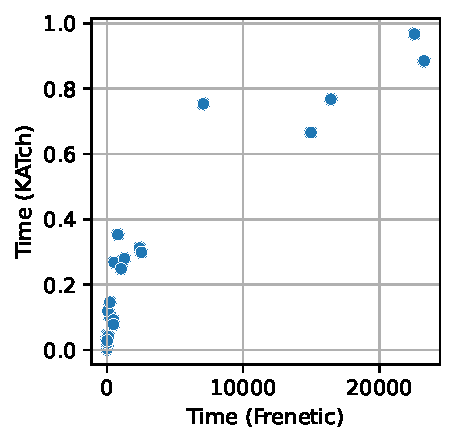
\includegraphics[scale=0.6]{plots/Topology Zoo_scatter.pdf}
    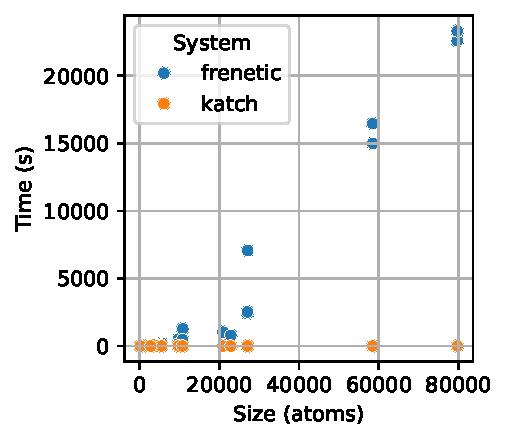
\includegraphics[scale=0.6]{plots/Topology Zoo_time_vs_size.pdf}
  \caption{Results of running \KATch{} and \Frenetic on Topology Zoo topologies.}\label{fig:topology-zoo}
\end{figure}

\subsection{Combinatorial Examples}

Finally, we ran experiments to test the hypothesis that \SPPs{} have
an asymptotic advantage for certain types of queries.  The key
advantage of \SPPs{} over \FDDs{} is that keeping the updates
associated with the fields themselves in the internal node allows
avoids a combinatorial blowup associated with sequencing. To test
this, we generated the following NetKAT programs:
\begin{description}
    \item[Inc:] Treating the input packet's $n$ boolean fields as a binary number, increment it by one.
    \item[Flip:] Sequentially flip the value of each of the $n$ boolean fields.
    \item[Nondet:] Set each field of the packet to a range of values from $0$ to $n$.
\end{description}
For Inc, we tested that repeatedly incrementing (using the $\star$
operator) can turn packet $00\cdots0$ into $11\cdots1$.  For Flip, we
tested that flipping all bits twice returns the original packet.  For
Nondet, we tested that setting the fields non-deteministically twice
is the same as doing it once.  The results of this experiment are
shown in \Cref{fig:combinatorial}.  Because the available fields are
hardcoded in \Frenetic, we only ran the Inc and Flip experiments up to
$n=10$. We ran the non-determinism test up to $n=15$.  \KATch{} can
finish all three queries up to $n=100$ in less than one minute,
demonstrating its aysmptotic advantage for these types of queries.

\begin{figure}
    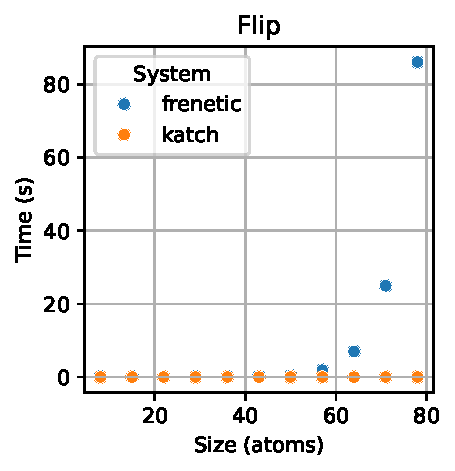
\includegraphics[scale=0.53]{plots/Flip_time_vs_size.pdf}
    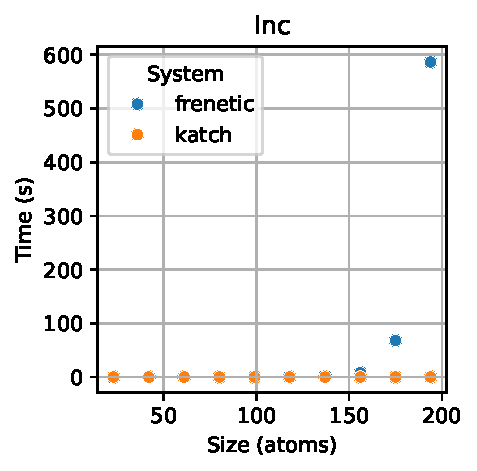
\includegraphics[scale=0.53]{plots/Inc_time_vs_size.pdf}
    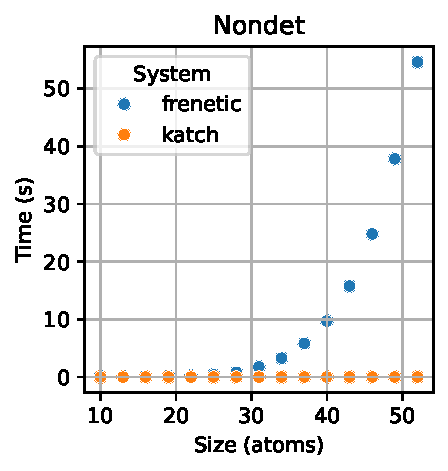
\includegraphics[scale=0.53]{plots/Nondet_time_vs_size.pdf}
  \caption{Results of running \KATch{} and \Frenetic on combinatorial benchmarks}\label{fig:combinatorial}
\end{figure}

\section{Related Work}

This section discusses the most closely related prior work to this
paper, focusing on three areas: network verification, NetKAT, and
automata-theoretic approaches to verification.

\paragraph*{Network Verification}
%
Early work by Xie et al.~\cite{Xie2005} proposed a unifying
mathematical model for Internet routers and developed algorithms for
analyzing network-wide reachability. Although the paper did not
discuss an implementation, its elegant formal model has been extremely
influential in the community and has served as the foundation for many
follow-on efforts, including this work. The emergence of
software-defined networking (SDN) led to a surge of interest in static
data plane verification, including systems such as Header Space
Analysis (HSA)~\cite{Kazemian2012}, Anteater~\cite{Mai2011},
VeriFlow~\cite{Khurshid2012}, Atomic Predicates
(AP)~\cite{Yang2016}. These systems all follow a common approach: they
build a model of the network-wide forwarding behavior and then check
whether given properties hold. However, they vary in the data
structures and algorithms used to represent and analyze the network
model. For instance, Anteater relies on first-order logic and SAT
solvers, while VeriFlow uses prefix trees and custom graph-based
algorithms. HSA and AP are arguably the most related to our work as
they use symbolic representations and BDDs respectively. However, they
still rely on ad hoc algorithms for network-wide analysis, which
differs from NetKAT's more principled approach based on
automata-theoretic foundations.

Another line of work has explored how to lift verification from the
data plane to the control plane. Batfish~\cite{Fogel2015,Brown2023}
proposed using symbolic simulation to analyze distributed control
planes---i.e., generating all possible data planes that might be
produced starting from a given control-plane configuration. Like
\KATch, Batfish uses a BDD-based representation for data plane
analysis. MineSweeper~\cite{Beckett2017} improves on Batfish using an
SMT encoding of the converged states of the control plane that avoids
having to explicitly simulate the underlying routing protocols. Recent
work has focused on using techniques like modular
reasoning~\cite{Tang2023,Thijm2023} abstract
interpretation~\cite{Beckett2020}, and a form of symmetry
reduction~\cite{Beckett2018} to further improve the scalability of
control-plane verification.

\paragraph*{\NetKAT}

\NetKAT was originally proposed as a semantic foundation for SDN data
planes~\cite{Anderson2014}. Indeed, being based on
KAT~\cite{Kozen1996}, the language provides a sound and complete
algebraic reasoning system. Later work on \NetKAT developed an
automata-theoretic (or coalgebraic) account of the
language~\cite{Foster2015}, including a decision procedure based on
bisimulation. However, the performance of this approach turns out to
be poor, as shown in our experiments, due to the use of ad hoc data
structures (``bases'') to encode packets and automata. \NetKAT's
compiler uses a variant of BDDs, called Forwarding Decision Diagrams
(FDDs), as well as an algorithm for converting programs to automata
using Antimirov derivatives~\cite{Smolka2015}. The \SPPn{}s proposed
in this paper improve on FDDs by ensuring uniqueness and supporting
efficient sequential composition in the common case. In addition, the
deterministic automata used in \KATch support additional ``negative''
operators that are useful for verification. Other papers based on
NetKAT have explored use of the language in other settings such as
distributed control planes~\cite{Beckett2016} and probabilistic
networks~\cite{Foster2016,Smolka2017,Smolka2019}. In the future, it
would be interesting to consider extending the techniques developed in
this paper to these richer settings. Another interesting direction for
future work is to build a symbolic verifier for the guarded fragment
of \NetKAT~\cite{Smolka20}.

\paragraph*{Automata-Theoretic Approach and Symbolic Automata}
%
Our work on \KATch builds on the large body of work on the
automata-theoretic approach to verification and symbolic automata. The
automata-theoretic approach was pioneered in the 1980s, with
applications of temporal logics and model checking to hardware
verification. BDDs, originally proposed by Lee \cite{Lee1959}, were
further developed by Bryant~\cite{Bryant1986}, and used by McMillan
for symbolic model checking~\cite{Burch1990}.

An influential line of work by D'Antoni and Veanus developed
techniques for representing and transforming finite automata where the
transitions are not labeled with individual characters but with
elements of a so-called effective Boolean
algebra~\cite{DAntoni2014,DAntoni2017}. Shifting from a concrete to a
symbolic representation requires generalizing classical algorithms,
such as minimization and equivalence, but facilitates building
automata and transducers that work over enormous alphabets, such as
Unicode.

Pous \cite{Pous2015} developed symbolic techniques for checking the
equivalence of automata where transitions are specified using
BDDs. The methods developed in this paper take Pous's work as a
starting point but, as highlighted in his paper, develop a non-trivial
extension to \NetKAT. In particular, \SPPn{}s provide a compact
representation for ``carry-on'' packets, which is a critical and
unique aspect of of \NetKAT's semantics. Bonchi and Pous
\cite{Bonchi2013} explored the use of up-to techniques for checking
equivalence of automata. In principle, one can view the
simplifications enforced by \KATch's term representations as a kind of
up-to technique, but a full investigation of this idea requires
additional work.

Our backward algorithm for computing bisimulations can be seen of a
variant of Moore's classic algorithm for computing the greatest
bisimulation to \NetKAT automata.  Doenges et al.~\cite{Doenges2022}
proposed an analogous approach for checking equivalence of automata
that model the behavior of P4 packet
parsers~\cite{Bosshart2014}. However, Leapfrog's model is simpler than
\NetKAT's, being based on classic finite automata, and it achieves
scalability primarily due to a novel up-to technique that ``leaps''
over internal buffering transitions rather than symbolic
representations.

\bibliographystyle{ACM-Reference-Format}
\bibliography{refs}

\end{document}
